\documentclass[11pt]{beamer}
\usepackage[spanish]{babel}

\mode<presentation> {
  \usetheme{Madrid}
}

\usepackage[spanish]{babel}
\usepackage[utf8]{inputenc}
\usepackage{graphicx} 
\usepackage{booktabs} 



\institute[CIMAT] 
{
%================= logos no meio =====================
%\vspace*{-0.35cm}

\includegraphics[scale=0.12]{img/cimat.png}

\includegraphics[width=1.8cm]{img/seminario_uam.png}
%\hspace*{0.25cm}~%
%\includegraphics[width=1.8cm]{img/logo-neo.png}
\vspace*{0.35cm}\\
Seminario del posgrado en matemáticas UAM-I \\
%\medskip
%\texttt{\{lods.eng,ronety\}@uea.edu.br} % emails
}
\date{\today}

\AtBeginSection[]
{
\begin{frame}
\frametitle{Contenido}
\tableofcontents[currentsection]
\end{frame}
}


\title[Seminario de UAM]
{Modelos de aprendizaje profundo}

\author[Suárez, M.A.]{Manuel Arturo Suárez Améndola}

\begin{document}
\begin{frame}
\titlepage 

\end{frame}

\begin{frame}
\frametitle{Contenido} 
\tableofcontents 
\end{frame}


\section{Antecedentes}
\begin{frame}{Motivación}
  \begin{block}{¿Cuál es el verdadero impacto de un derrame de petróleo?}
    \begin{itemize}
      \item Consecuencias ambientales
      \item Consecuencias sociales
      \item Consecuencias económicas
    \end{itemize}
  \end{block}

\end{frame}

\begin{frame}{Pozos perforados (2011 - 2013)}
    \begin{figure}
        \centering
        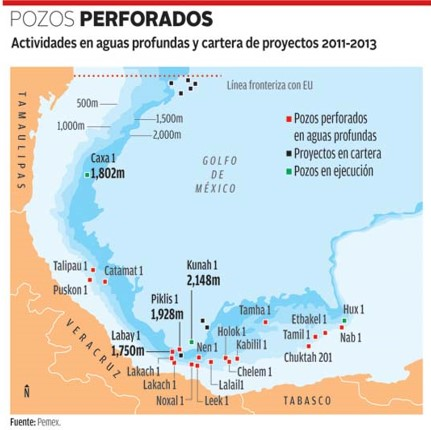
\includegraphics[scale=0.4]{img/section_01/pozos_perforados_2013.jpg}
        \caption{Actividades de exploración y perforación en 2013}
        \label{fig:section_01_pozos}
    \end{figure}
\end{frame}

\begin{frame}{Infraestructura Petrolera 2015)}
    \begin{figure}
        \centering
        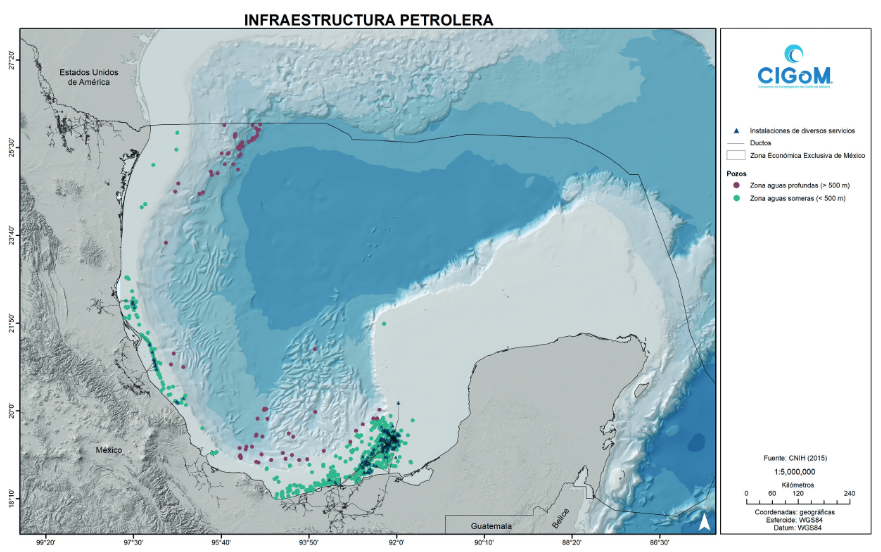
\includegraphics[scale=0.3]{img/section_01/infraestructura_petrolera}
        \caption{Infraestructura petrolera de exploración, extracción y producción de gas petróleo en la Zona Económica Exclusiva mexicana. Fuente: Atlas de Línea Base Ambiental del Golfo de México, Tomo IV, CIGOM}
        \label{fig:section_01_infraestructura}
    \end{figure}
\end{frame}

\begin{frame}{Deep Water Horizon}
    \begin{figure}
        \centering
        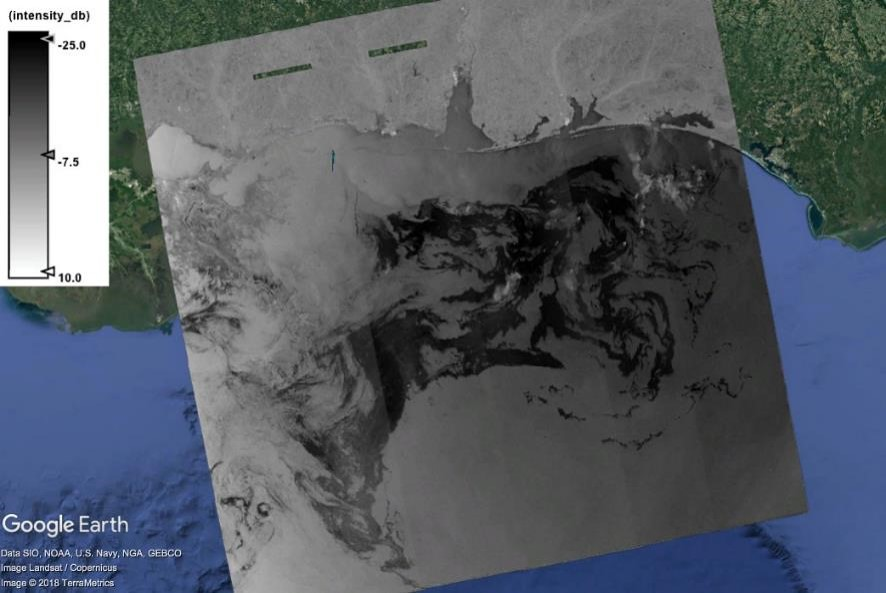
\includegraphics[scale=0.3]{img/section_01/deep-water-horizon.jpg}
        \caption{Extensión del derrame}
        \label{fig:section_01_deep_water_horizon}
    \end{figure}

    Estimación del derrame: 779,000 toneladas de crudo.
\end{frame}

\begin{frame}{Deep Water Horizon - Timelime}
  \begin{figure}
    \centering
    \begin{tikzpicture}[scale=0.5,every node/.style={outer sep=5pt}]
      %Notation: {year, the title of the event}
      %NOTE! Everyting is zero-based
      \footnotesize
      \def\ourInfo{{
        {"April 20, 2010","At 10 p.m. (CT) an explosion and fire ocurred on the \\ Deepwater Horizon drilling rig."},
        {"April 22, 2010","10:30 a.m. (CT), the Deepwater Horizon drilling rig \\ sank to the bottom of the Gulf of Mexico."},
        {"May 2, 2010","Relief well. An additional 30 vessels and 1,000 responders \\were deployed to the Gulf Coast."},
        {"June 6, 2010","Tests confirmed that tarballs from the Deepwater had \\washed ashore in all five Gulf states."},
        {"July 10, 2010","At 2:25 p.m. (CT), BP closes the valves on the cap \\and stops the oil leaking out of the riser."}
      }}
      \pgfmathsetmacro{\length}{4}% Zero based.

      % Loop through the array containing all events.
      \foreach \i in {0, ..., \length}{
          \pgfmathsetmacro{\year}{\ourInfo[\i][0]}% Get the left cell (year)
          \pgfmathsetmacro{\eventName}{\ourInfo[\i][1]}% Get the right cell (event name)
          \draw[thick,red] (0,-2*\i-2)--(0,-2*\i);% Draw vertical line
          \ifnum \i=1 % Should be in red text
            \draw(0,-2*\i-1) node[red, right, align = left]{\eventName};% Display the event name
            \draw(0,-2*\i-1) node[red, left] {\year};
          \else % Should be in black text
             \draw(0,-2*\i-1) node[right, black, align = left]{\eventName};% Display the event name
             \draw(0,-2*\i-1) node[left] {\year};% Display the year
          \fi
      }
      % Draw the bullet with the dash
      \foreach \i in {0, ..., \length}{
          \filldraw[draw = white, fill = red,thick] (0,-2*\i-1) circle (5pt);
          \draw[thick,red] (-12pt,-2*\i-1)--(0,-2*\i-1);
      }
    \end{tikzpicture}
    \caption{Línea de tiempo del evento. Fuente: \url{https://response.restoration.noaa.gov/timelines/10-years-ago-deepwater-horizon-oil-spill}}
  \end{figure}
  \footnotesize
  \footnote{}
\end{frame}

\begin{frame}{Ixtoc I}    
    \begin{figure}
        \centering
        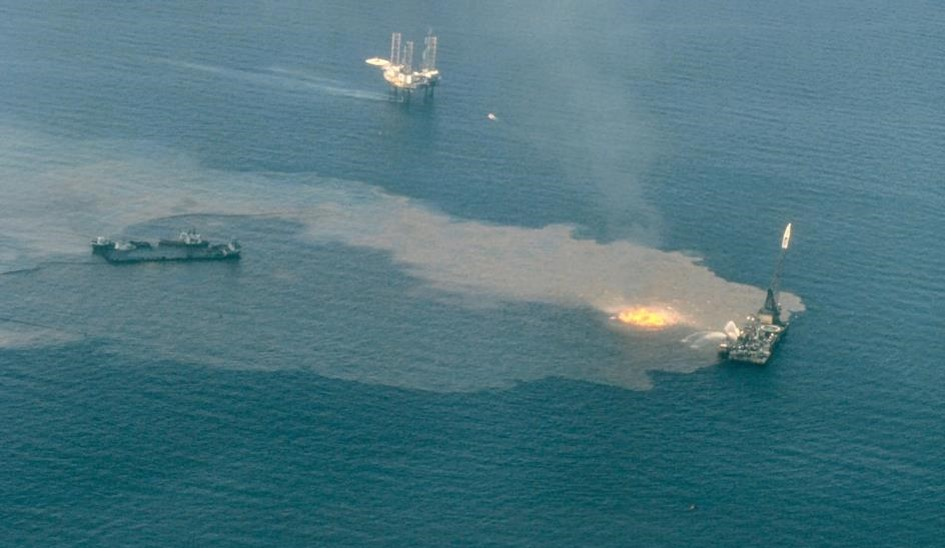
\includegraphics[scale=0.3]{img/section_01/explosion_ixtoc.jpg}
        \caption{Explosión del pozo Ixtoc I, Sonda de Campeche, 3 de junio de 1979}
        \label{fig:section_01_explosion_ixtoc}
    \end{figure}

    Estimación del derrame, 530,000 toneladas de crudo.
\end{frame}

\begin{frame}{Ek Balam}    
    \begin{figure}
        \centering
            \begin{tabular}[c]{cc}
              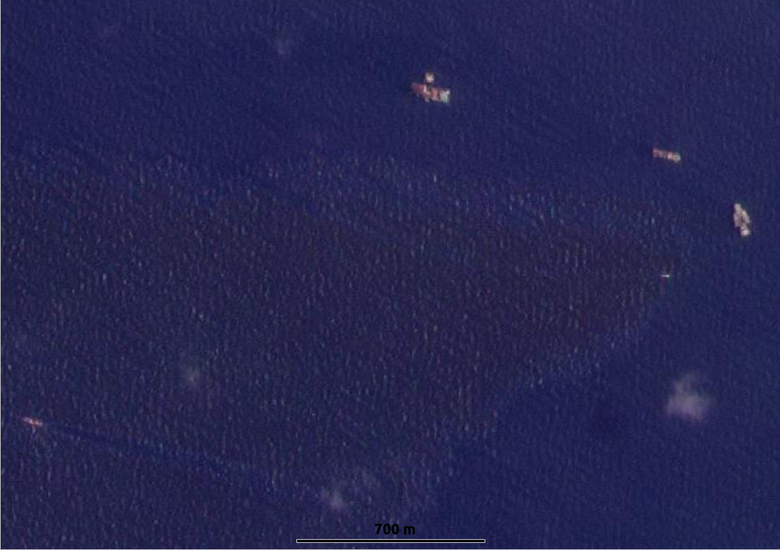
\includegraphics[scale=0.2]{img/section_01/ek_balam-6-julio.png}&
              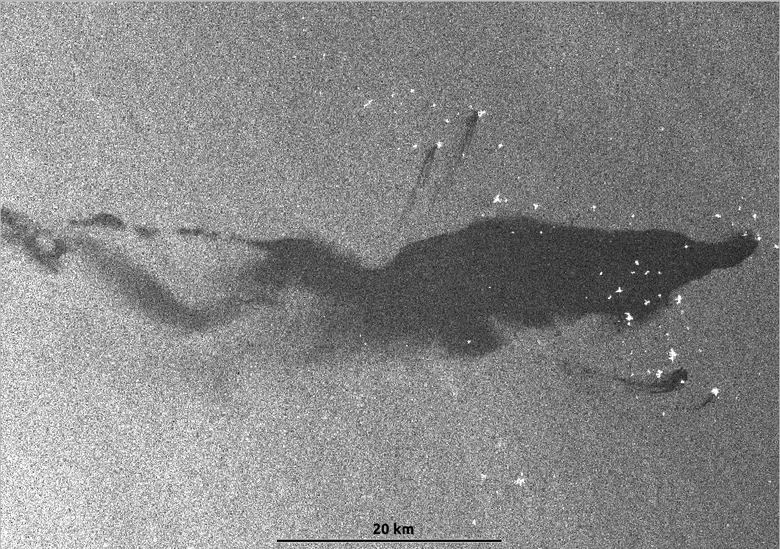
\includegraphics[scale=0.2]{img/section_01/ek_balam-12-julio.png}\\
            \end{tabular}
        \caption{Derrame en la Sonda de Campeche, Julio 2023}
        \label{fig:section_01_explosion_ixtoc}
    \end{figure}
\end{frame}

\begin{frame}{Dinámica de la interacción océano-petróleo}
    \footnotesize
    \begin{block}{Diferentes procesos físicos y químicos dificultan el tratamiento}
      \begin{itemize}
        \item Dispersión
        \item Evaporación
        \item Emulsión
        \item Sedimentación
      \end{itemize}
    \end{block}
    \begin{figure}
      \centering
      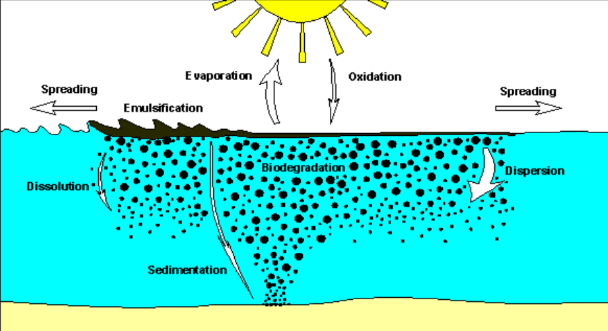
\includegraphics[scale=0.3]{img/section_01/dinamica-derrame.png}
      \caption{Dinámica de la interacción}
      \label{fig:section_01_dinamica_derrame}
    \end{figure}    
\end{frame}


\section{Revisión del Estado del Arte}
\begin{frame}{Review}
  \begin{block}{Sensors, Features, and Machine Learning for Oil Spill Detection and Monitoring: A Review \cite{rs12203338}}
    \textit{Remote sensing technologies and machine learning (ML) algorithms play an increasingly   important role in accurate detection and monitoring of oil spill slicks, assisting scientists in forecasting their trajectories, developing clean-up plans, taking timely and urgent actions, and applying effective treatments to contain and alleviate adverse effects. Review and analysis of different sources of remotely sensed data and various components of ML classification systems for oil spill detection and monitoring are presented in this study. More than 100 publications in the field of oil spill remote sensing, published in the past 10 years, are reviewed in this paper.}
  \end{block}  
\end{frame}

\begin{frame}{Marco de trabajo - características}
  \footnotesize
  Marco general de trabajo
  \begin{figure}
      \centering
      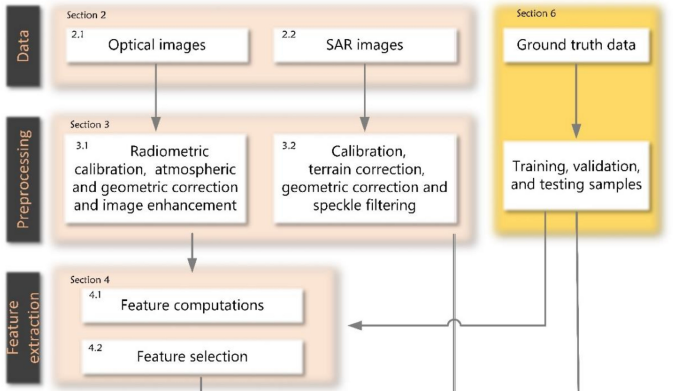
\includegraphics[scale=0.6]{img/section_02/framework_spill_detection.png}
      \caption{Preprocesamiento y extracción de características \cite{rs12203338}}
      \label{fig:preprocessing_and_feature_extraction}
  \end{figure}
\end{frame}

\begin{frame}{Marco de trabajo - algoritmos}
  \begin{figure}
      \centering
      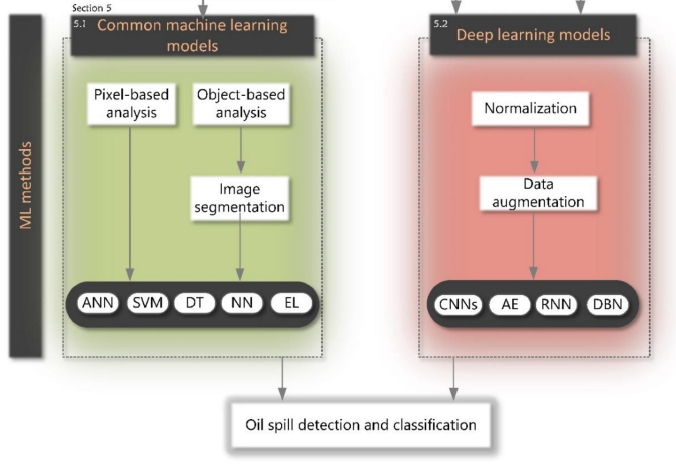
\includegraphics[scale=0.6]{img/section_02/framework_spill_detection2.png}
      \caption{Algoritmos de detección y clasificación \cite{rs12203338}}
      \label{fig:my_label}
  \end{figure}
\end{frame}

\begin{frame}{Imágenes ópticas}
  \begin{figure}
      \centering
      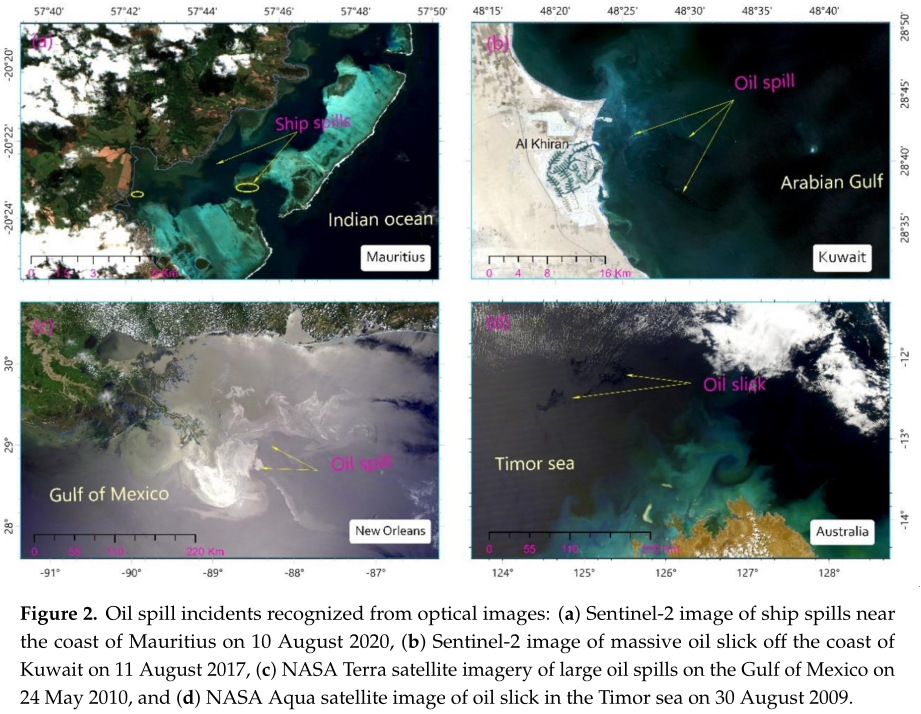
\includegraphics[scale=1.2]{img/section_02/caracteristicas_opticas_01.png}
      \caption{Imágenes multiespectrales}
      \label{fig:optical_features_01}
  \end{figure}
\end{frame}

\begin{frame}{Satélites ópticos}
  \begin{figure}
      \centering
      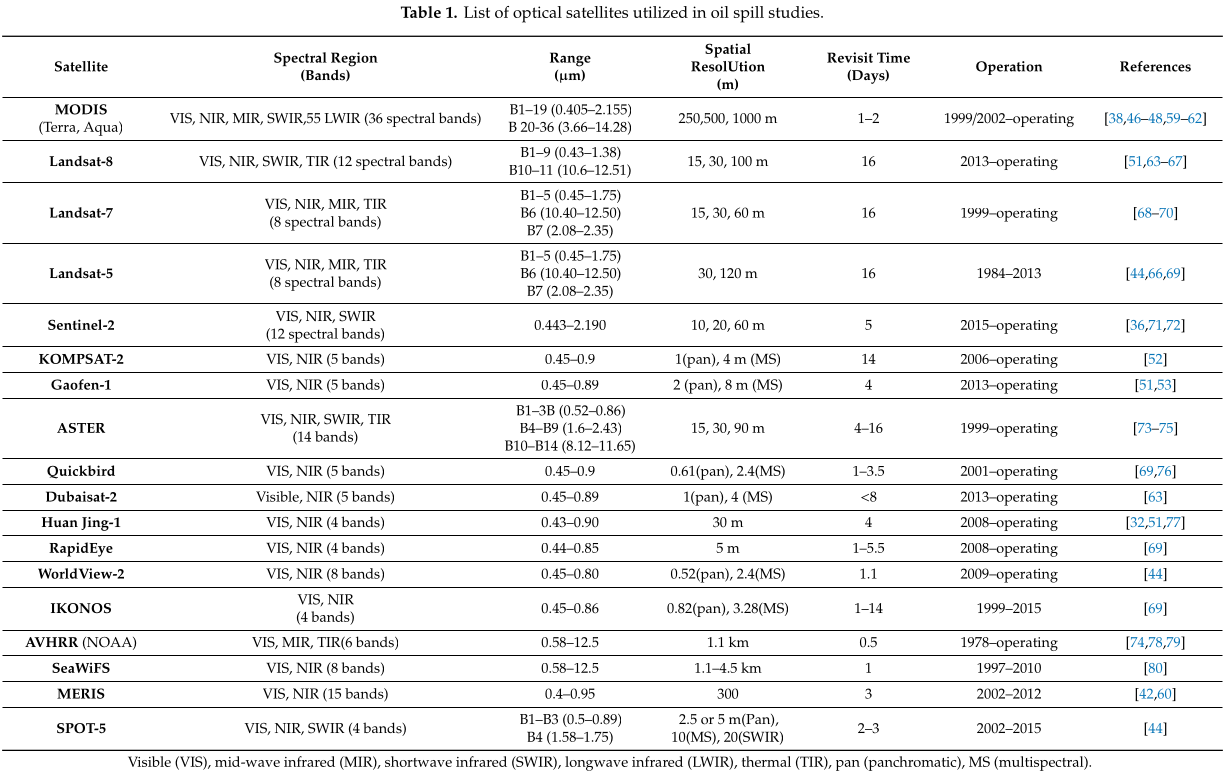
\includegraphics[scale=1.0]{img/section_02/caracteristicas_opticas_02.png}
      \caption{Lista de satélites multiespectrales e hiperespectrales usados}
      \label{fig:optical_features_02}
  \end{figure}
\end{frame}

\begin{frame}{Imágenes radar}
  \begin{figure}
      \centering
      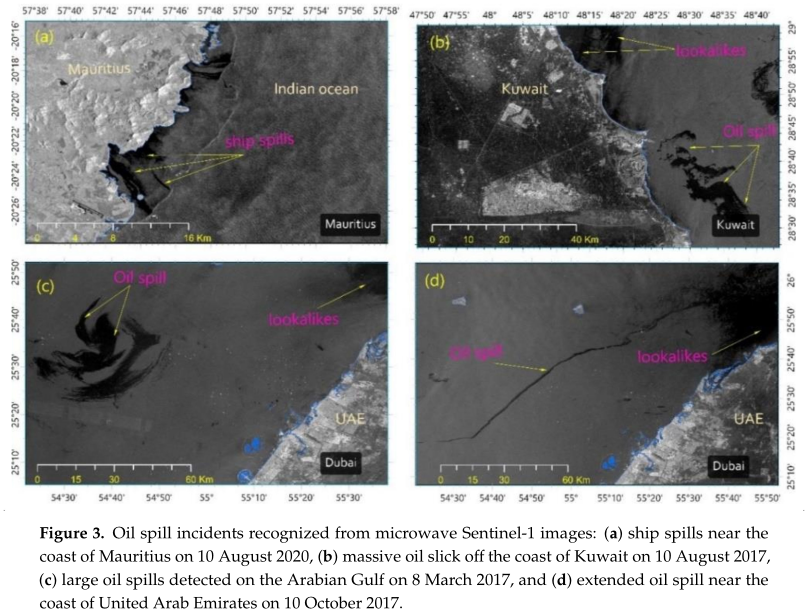
\includegraphics[scale=1.2]{img/section_02/caracteristicas_radar_01.png}
      \caption{Imágenes de radar}
      \label{fig:optical_features_01}
  \end{figure}
\end{frame}

\begin{frame}{Satélites de radar}
  \begin{figure}
      \centering
      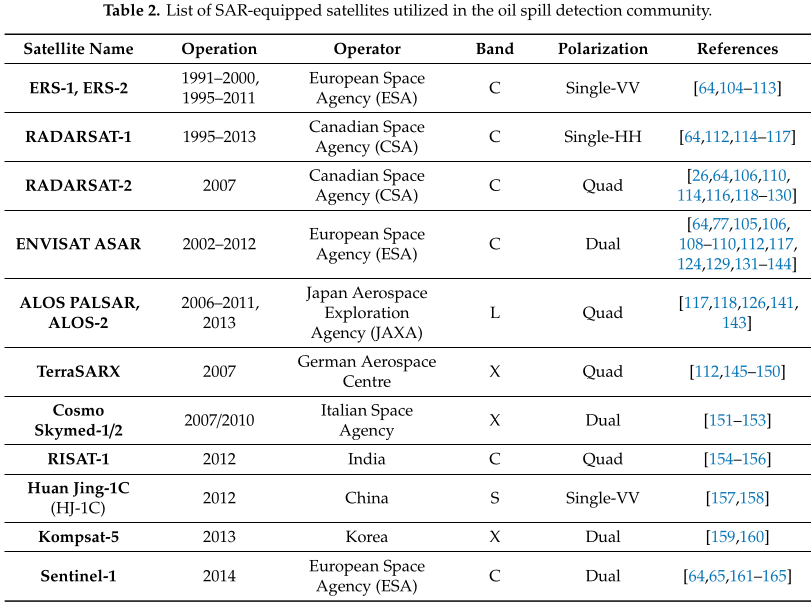
\includegraphics[scale=1.2]{img/section_02/caracteristicas_radar_02.png}
      \caption{Lista de satélites radar}
      \label{fig:optical_features_01}
  \end{figure}
\end{frame}

\begin{frame}{Extracción de características I}
  \begin{figure}
      \centering
      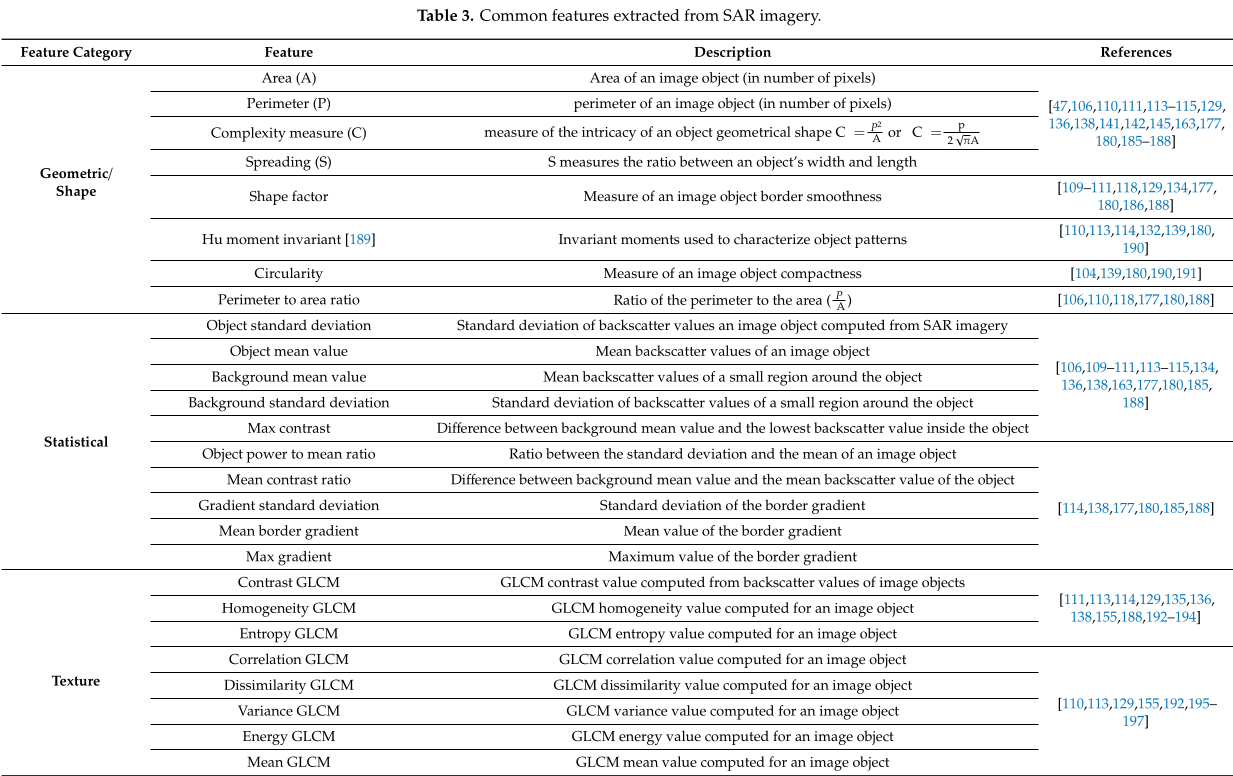
\includegraphics[scale=1.0]{img/section_02/tabla_caracteristicas_01.png}
      \caption{Características geométricas, estadísticas y de textura}
      \label{fig:optical_features_01}
  \end{figure}
\end{frame}

\begin{frame}{Extracción de características II}
  \begin{figure}
      \centering
      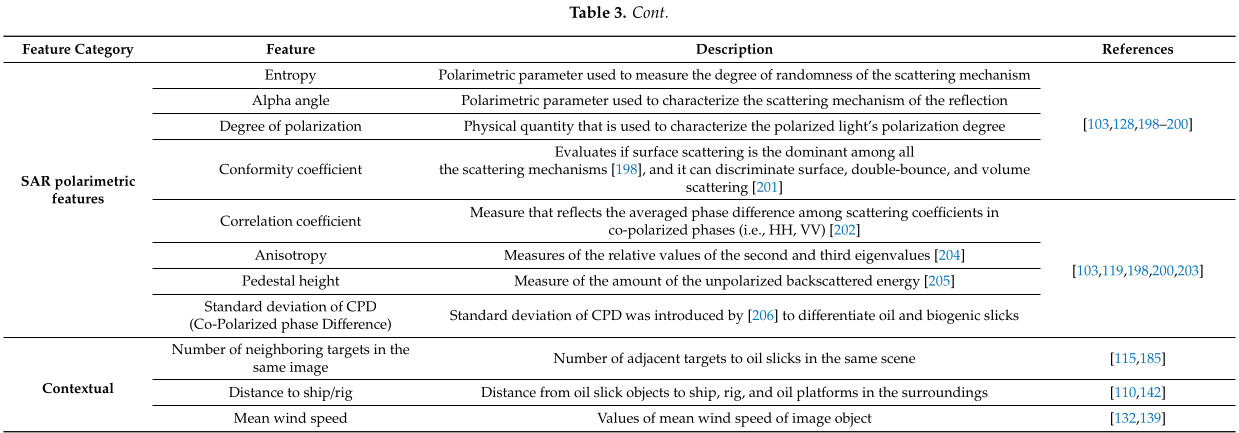
\includegraphics[scale=1.0]{img/section_02/tabla_caracteristicas_02.png}
      \caption{Características polarimétricas y contextuales}
      \label{fig:optical_features_01}
  \end{figure}
\end{frame}

\begin{frame}{Extracción de características III}
  \begin{figure}
      \centering
      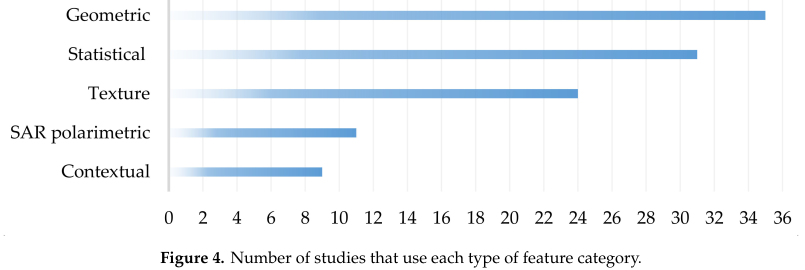
\includegraphics[scale=1.0]{img/section_02/tabla_caracteristicas_03.png}
      \caption{Cantidad de artículos por característica empleada}
      \label{fig:optical_features_01}
  \end{figure}
\end{frame}

\begin{frame}{Algoritmos clásicos de aprendizaje máquina}
    \begin{figure}
        \centering
        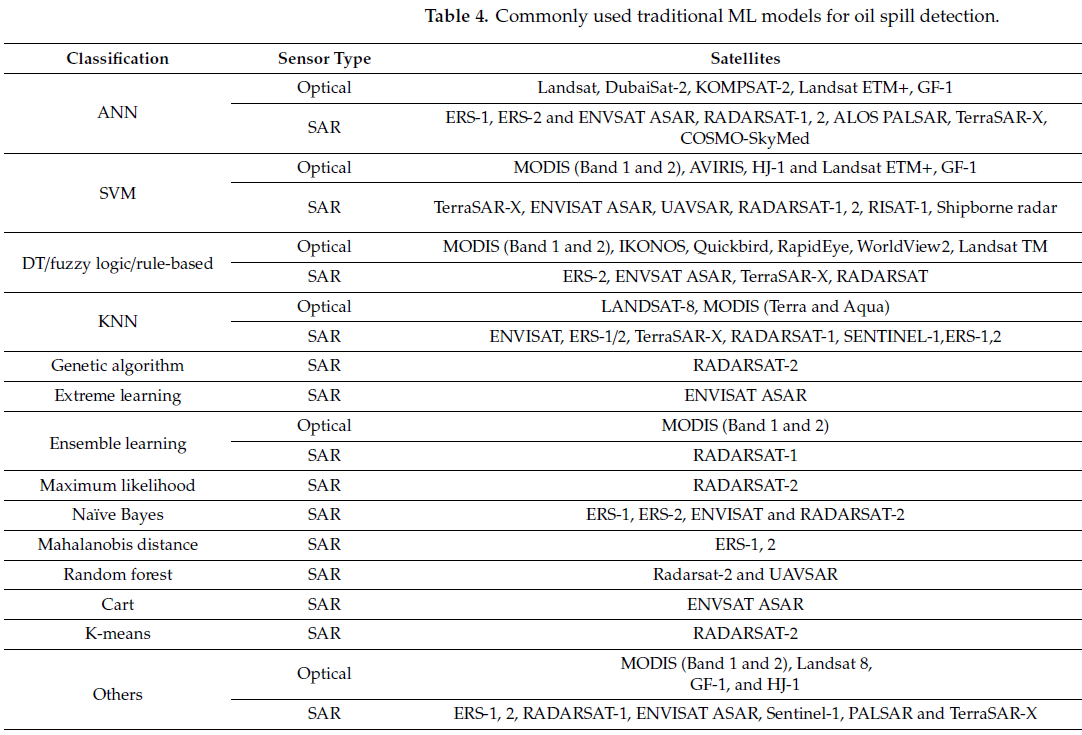
\includegraphics[scale=0.4]{img/section_02/oil_spill_detection_machine_learning.png}
        \caption{Classical Machine Learning}
        \label{fig:my_label}
    \end{figure}
\end{frame}

\begin{frame}{Algoritmos clásicos de aprendizaje máquina}
    \begin{figure}
        \centering
        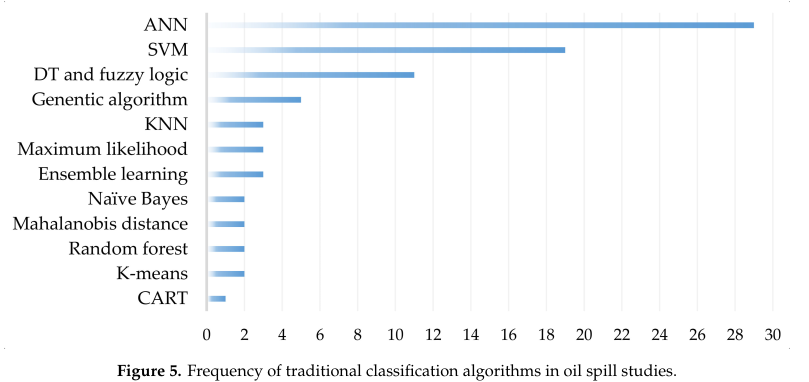
\includegraphics[scale=1.2]{img/section_02/frecuencias_machine_learning.png}
        \caption{Número de artículos por algoritmo}
        \label{fig:my_label}
    \end{figure}
\end{frame}

%\begin{frame}{Arquitectura de la CNN}
%    \begin{figure}
%        \centering
%        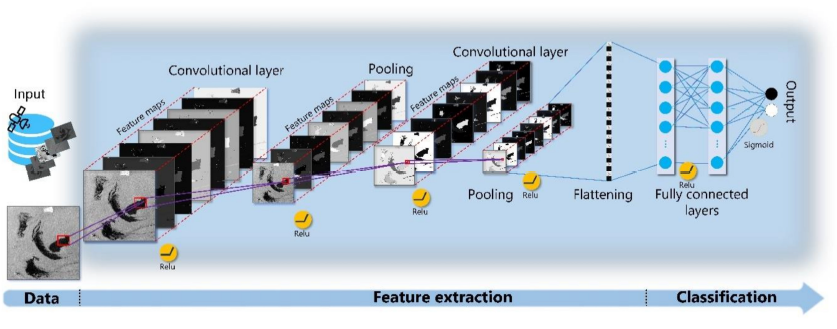
\includegraphics[scale=0.7]{img/section_02/oil_spill_detection_cnn_framework.png}
%        \caption{Convolutional Neural Network \cite{rs12203338}}
%        \label{fig:my_label}
%    \end{figure}
%\end{frame}

\begin{frame}{Algoritmos de aprendizaje profundo I}
    \begin{figure}
        \centering
        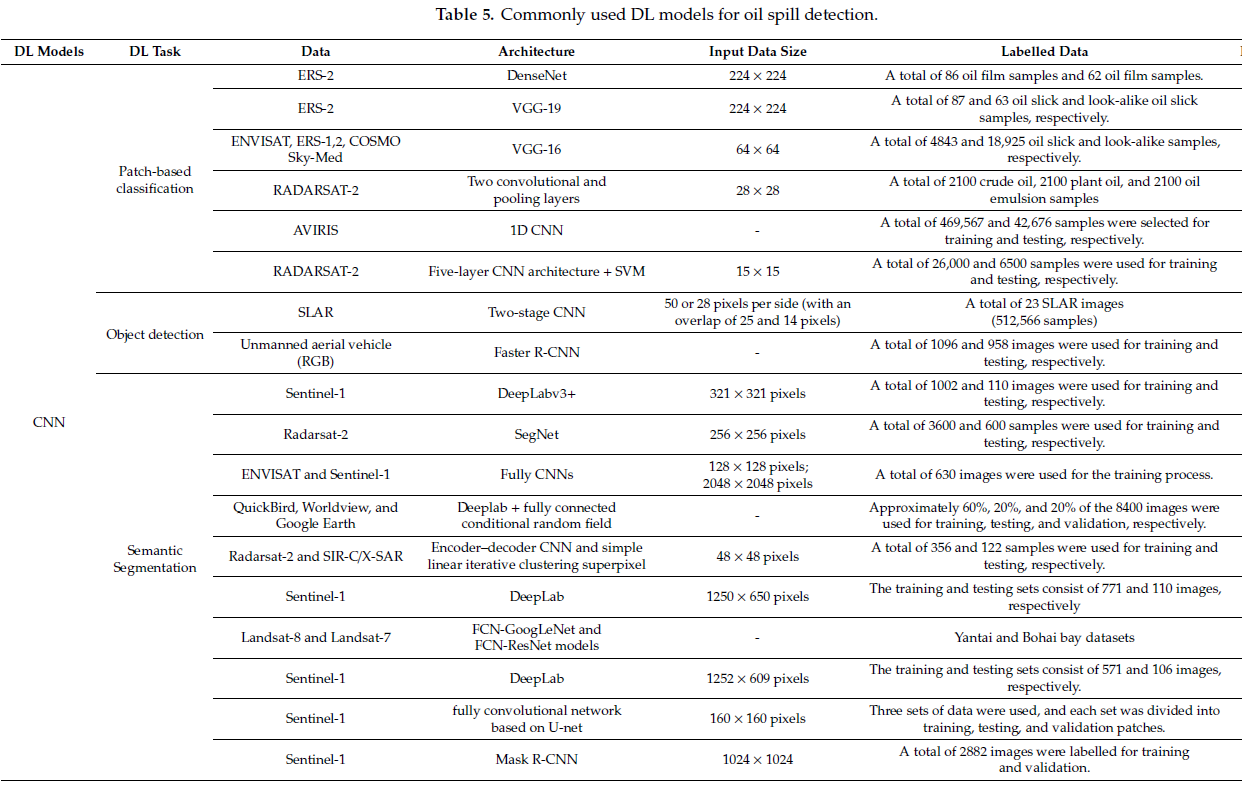
\includegraphics[scale=0.4]{img/section_02/oil_spill_detection_deep_learning.png}
        \caption{Deep Learning \cite{rs12203338}}
        \label{fig:my_label}
    \end{figure}
\end{frame}

\begin{frame}{Algoritmos de aprendizaje profundo II}
    \begin{figure}
        \centering
        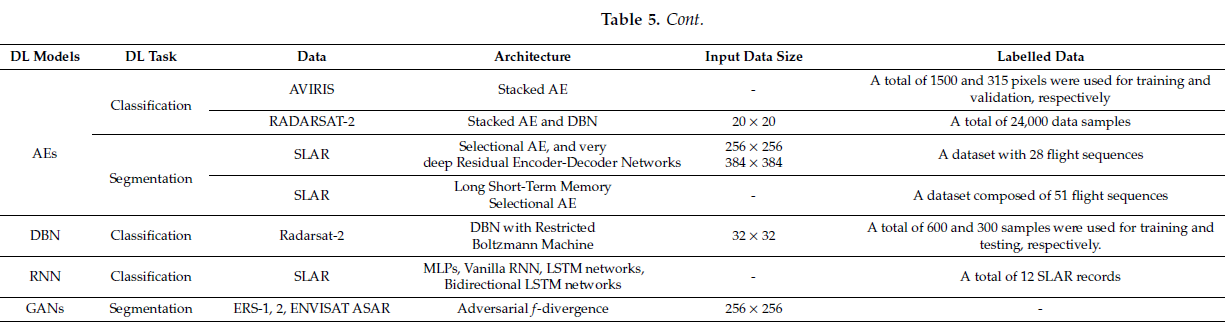
\includegraphics[scale=0.5]{img/section_02/oil_spill_detection_deep_learning2.png}
        \caption{Deep Learning \cite{rs12203338}}
        \label{fig:my_label}
    \end{figure}
\end{frame}




\section{Percepción Remota}
\begin{frame}{Percepción Remota}
    \begin{block}{¿Qué es la percepción remota?}
        Técnica o conjunto de técnicas que permite medir y registrar la energía
        electromagnética reflejada o emitida por la superficie de la Tierra y 
        relacionar tales mediciones con su naturaleza y distribución.
    \end{block}    

    \begin{figure}
      \begin{center}
        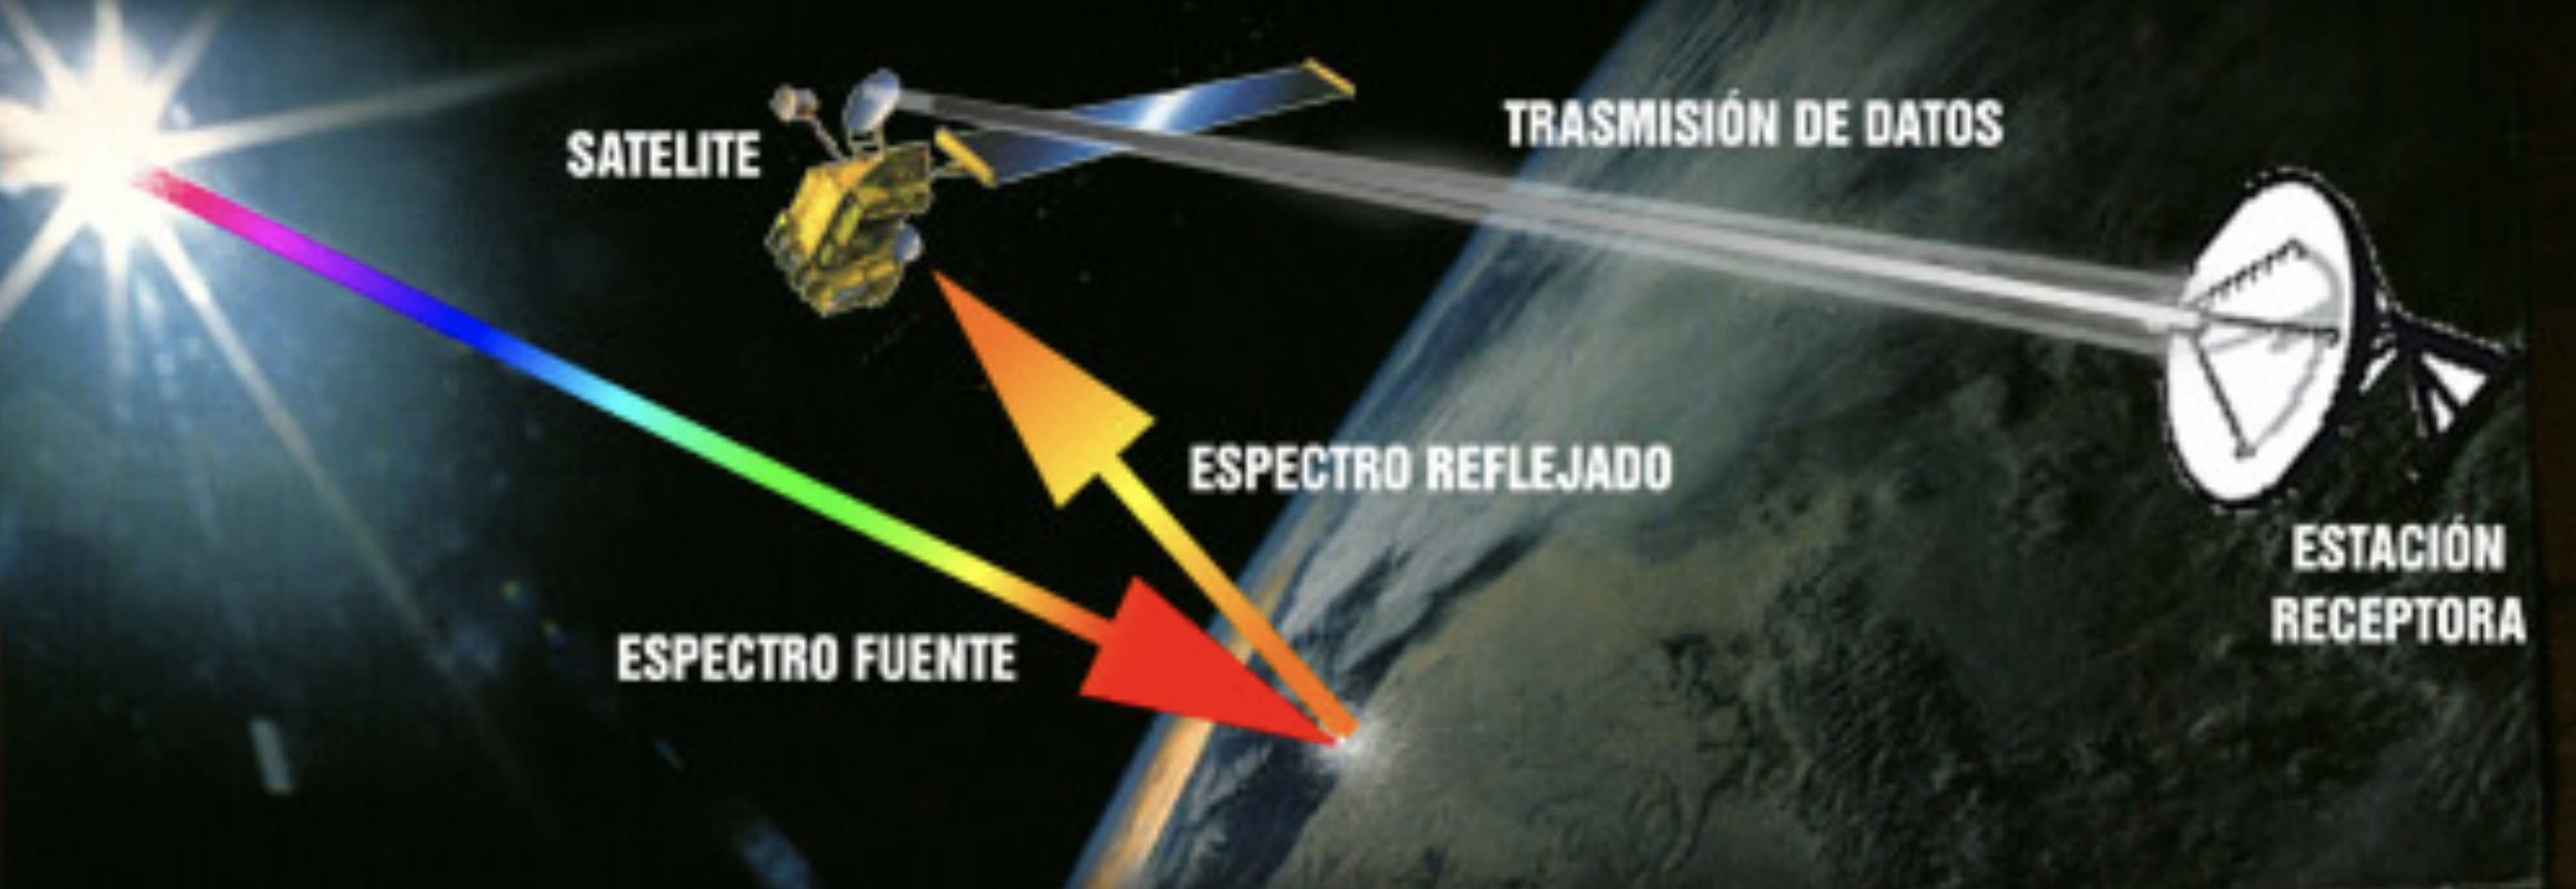
\includegraphics[width=0.95\textwidth]{img/section_03/percepcion_remota}
      \end{center}
      \caption{Fuente: \url{https://haciaelespacio.aem.gob.mx/revistadigital/articul.php?interior=706}}\label{fig:percepcion_remota}
    \end{figure}
    
\end{frame}

\begin{frame}{Sistemas de percepción remota}
  \begin{figure}
    \begin{center}
      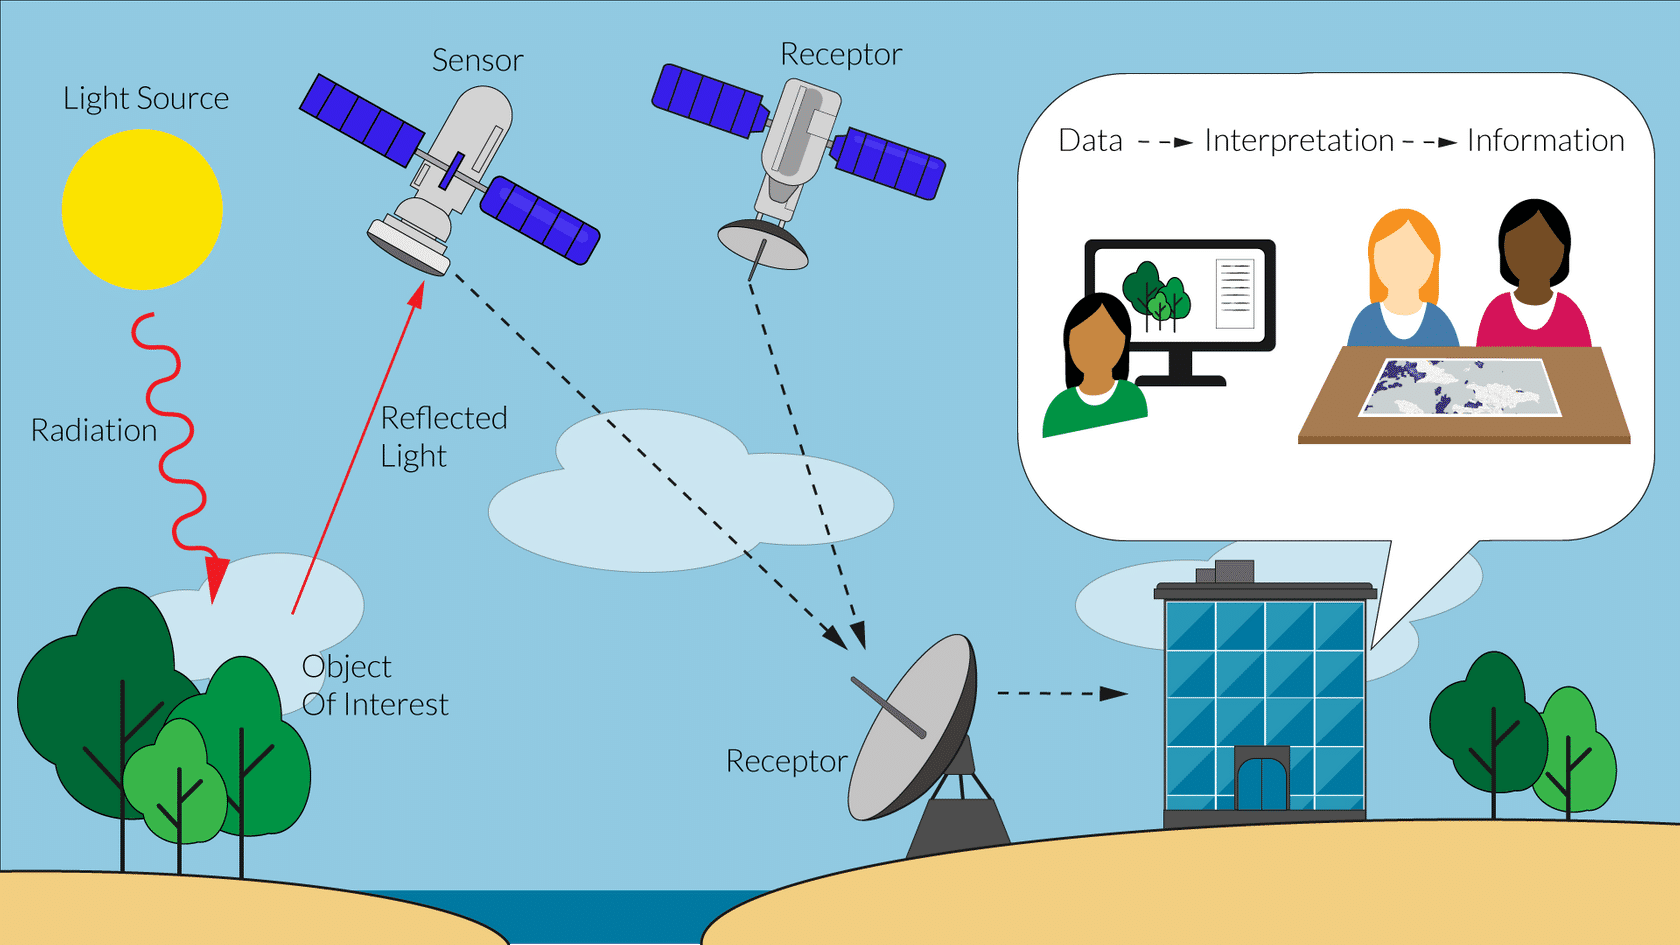
\includegraphics[width=0.95\textwidth]{img/section_03/elementos3.jpg}
    \end{center}
    \caption{Elementos de un sistema de percepción remota}
    \label{fig:elementos_percepcion_remota}
  \end{figure}
\end{frame}
  

\begin{frame}{Tipos de sensores}
    \begin{itemize}
        \item Sensores pasivos.- no poseen una fuente de energía por lo que solo detectan la radiación emitida y/o reflejada por la superficie terrestre que proviene de una fuente externa (como el la luz del sol).
        \item Sensores activos.- poseen una fuente propia de energía que les permite emitir su propia radiación la cuál interactúa con la superficie terrestre y al ser reflejada es captada por el sensor.
    \end{itemize}
    
    \begin{figure}
        \centering
        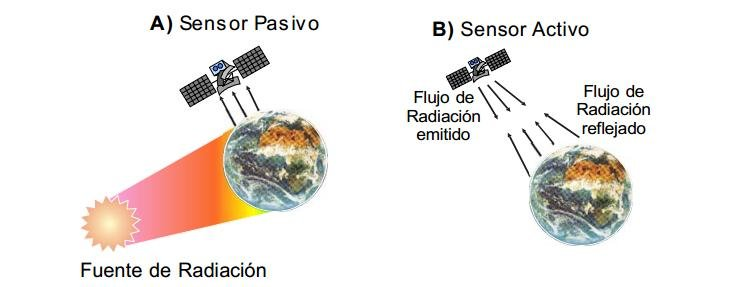
\includegraphics[scale=0.4]{img/section_03/tipos_de_sensores.png}
        \caption{Sensores activos y sensores pasivos \cite{phdthesis}}
        \label{fig:section_03_sensores_activos_pasivos}
    \end{figure}
\end{frame}

\begin{frame}{Espectro eletromagnético}
    \begin{figure}
        \centering
        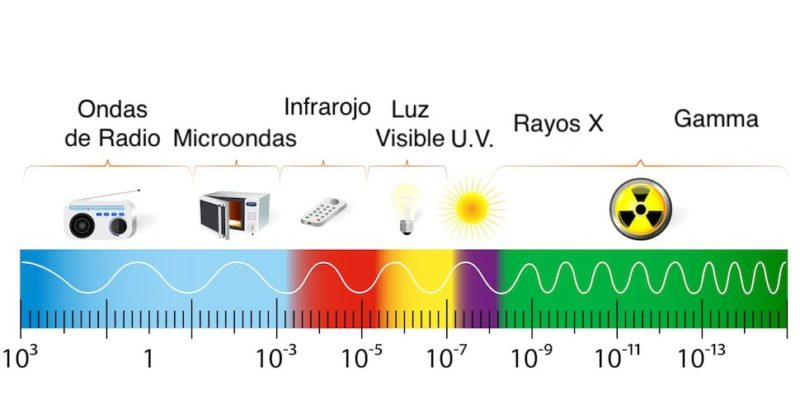
\includegraphics[scale=0.2]{img/section_03/espectro-electromagnetico.jpg}
        \caption{Espectro electromagnético}
        \label{fig:section_03_espectro_electromagnetico}
    \end{figure}
    
    \tiny
    \begin{table}
        \centering
        \begin{tabular}{c|c|c}
            \hline
            Banda & Longitud de onda & Tipo de Instrumentos \\
            \hline
            Radar & 1-30 cm & SLAR/SAR \\
            Microondas & 2-8 mm & Radiómetros \\
            Infrarojo termal & 1-14 um & Videocámaras y escáner de línea \\
            Infrarojo (MIR) & 3-5 um & Videocámaras y escáner de línea \\
            Bajo infrarojo & 1-3 um & Filme y videocámaras \\
            Visual & 350-750 nm & Filme, videocámaras y espectrómetros \\
            Ultravioleta & 250-350 nm & Filme, videocámaras y escáner de línea \\
            \hline
        \end{tabular}
        \caption{Bandas en detección remota}
        \label{tab:bandas_deteccion_remota}
    \end{table}
\end{frame}

\begin{frame}{Resolución}
    
  \begin{block}{Resolución de los sensores remotos}
    La resolución de un sensor es su habilidad para registrar información en detalle de las distintas cubiertas. La resolución depende de la capacidad de los sensores para distinguir variaciones de la energía electromagnética, del detalle espacial que captura y del número y ancho de las bandas que alberga.
  \end{block}
 \end{frame}
    
\begin{frame}{Resolución espacial}
  \begin{block}{Resolución espacial}
    es el objeto más pequeño que puede ser distinguido sobre la imagen. Define el tamaño del píxel, que es la distancia correspondiente al tamaño de la mínima unidad de información en la imagen.
  \end{block}

  \begin{figure}
    \begin{center}
      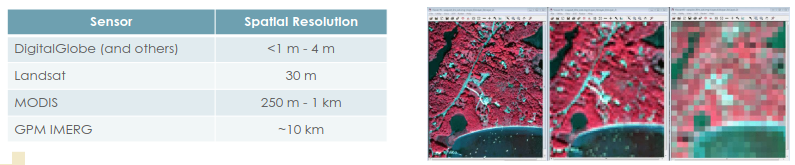
\includegraphics[width=0.95\textwidth]{img/section_03/resolucion_espacial}
    \end{center}
    \caption{Fuente: Fundamentals of Remote Sensing - NASA Applied Sciences}
    \label{fig:resolucion_multiespectral_vs_hiperespectral}
  \end{figure}
\end{frame}

\begin{frame}{Resolución espectral}
  \begin{block}{Resolución espectral}
    es el número y el ancho de las bandas espectrales que puede discriminar el sensor, monoespectrales y multiespectrales. Típicamente un sensor multiespectral tiene de 3 a 10 bandas mientras que uno hiperespectral puede contener cientos de ellas.
  \end{block}

  \begin{figure}
    \begin{center}
      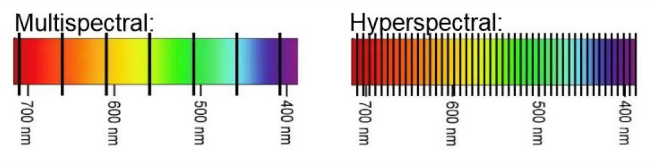
\includegraphics[width=0.95\textwidth]{img/section_03/resolucion_espectral}
    \end{center}
    \caption{Fuente: Fundamentals of Remote Sensing - NASA Applied Sciences}
    \label{fig:resolucion_espectral}
  \end{figure}
  
\end{frame}

\begin{frame}{Resolución radiométrica}
  \begin{block}{Resolución radiométrica}
    es la capacidad para detectar variaciones en la radiancia espectral que recibe. Determina el número de niveles de gris recogidos y se expresa en niveles por píxel. A mayor resolución radiométrica, mejor interpretación de la imagen.
  \end{block}

  \begin{figure}
    \begin{center}
      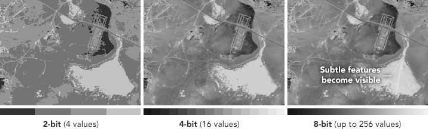
\includegraphics[width=0.80\textwidth]{img/section_03/resolucion_radiometrica}
    \end{center}
    \caption{Fuente: Fundamentals of Remote Sensing - NASA Applied Sciences}
    \label{fig:resolucion_radiometrica}
  \end{figure}
\end{frame}

\begin{frame}{Resolución temporal}
  \begin{block}{Resolución temporal}
    es la periodicidad con que el sensor adquiere imágenes de la misma porción de la superficie terrestre. Esta en función de las características orbitales de la plataforma (altura, velocidad e inclinación) y del diseño del sensor (ángulo de observación y ángulo de cobertura).
  \end{block}

  \begin{figure}
    \begin{center}
      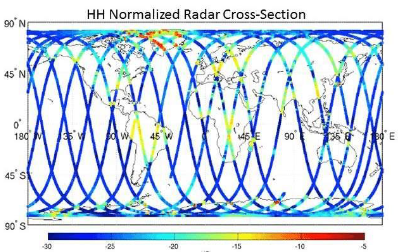
\includegraphics[scale=0.4]{img/section_03/resolucion_temporal}
    \end{center}
    \caption{Fuente: Fundamentals of Remote Sensing - NASA Applied Sciences}
    \label{fig:resolucion_temporal}
  \end{figure}
\end{frame}

\begin{frame}{Radar de Apertura Sintética}
    \footnotesize
    
    \begin{itemize}
        \item Sensor activo.- emite microondas ($f_0 = 1-30 Ghz$) con cierto ángulo de incidencia ($\theta_i = 20-65°$) y forma imágenes con el eco $\sigma^0$ de la radiación emitida.

        \item Apertura sintética.- integra la historia de $\sigma^0$ durante un cierto tiempo $T_i$ a lo largo de la trayectoria de vuelo del sensor y con ello \textit{sintetiza} una antena $L_{SAR} >> L_{real}$

        \item Formación de la imagen.- basada en el principio de retrodispersión de las microondas por parte de las ondas de Bragg.
    \end{itemize}

    \begin{figure}
        \centering
        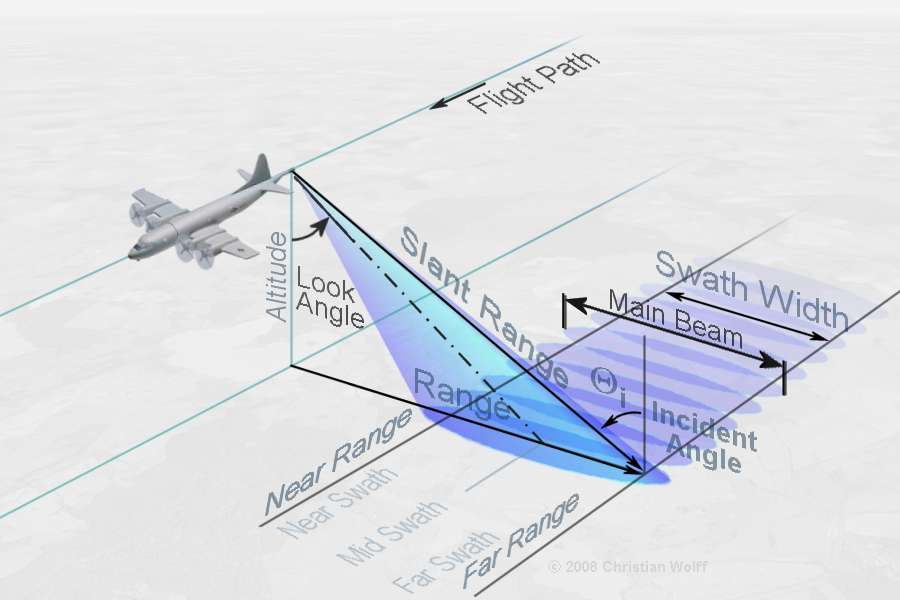
\includegraphics[scale=0.2]{img/section_03/SLAR-geometry_p.jpg}
        \caption{Radar de apertura sintética}
        \label{fig:section_03_radar_apertura_sintetica}
    \end{figure}
\end{frame}

\begin{frame}{Principios de formación de la imagen de radar}
  \begin{block}{Fundamento básico}
    El fundamento básico de una imagen de radar es un sensor que emite un pulso y a través de la diferencia en el transcurso de tiempo entre su emisión y recepción así como de la amplitud del pulso retornado, se puede obtener la distancia del sensor a la que se encuentra el objeto en el que rebotó el pulso.
  \end{block}

  \begin{figure}
    \begin{center}
      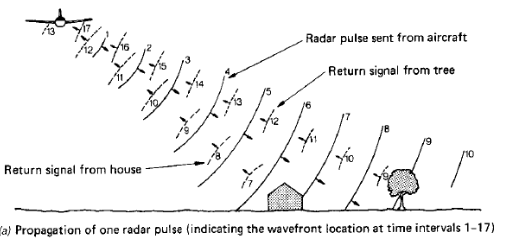
\includegraphics[scale=0.4]{img/section_03/principio_01}
    \end{center}
    \caption{Fuente: Fundamentos de teledetección radar. Gobierno de España}
    \label{fig:resolucion_temporal}
  \end{figure}
\end{frame}

\begin{frame}{Frecuencias de operación}
  \begin{block}{Frecuencias}
    Los radares trabajan en la frecuencia del espectro electromagnético de las microondas (por lo que también son llamados sensores de microondas) pero se subdividen en los siguientes grupos
  \end{block}

  \footnotesize
  \begin{table}
    \caption{Longitudes de onda y frecuencias de radar}
    \label{tab:longitudes_onda}
    \begin{center}
      \begin{tabular}[c]{c|l|l}
        \hline
        Banda & Longitud de onda (cm) & Frecuencia (GHz) \\
        \hline
        Ka & 0.75 - 1.2 & 40 - 25 \\
        K & 1.2 - 1.67 & 25 - 18 \\
        Ku & 1.7 - 2.5 & 17.6 - 12 \\
        X & 2.5 - 4 & 12 - 7.5 \\
        C & 4 - 8 & 7.5 - 3.75 \\
        S & 8 - 15 & 3.75 - 2 \\
        L & 15 - 30 & 2 - 1 \\
        P & 60 - 120 & 0.5 - 0.25 \\
        \hline
      \end{tabular}
    \end{center}
  \end{table}
\end{frame}
  


\begin{frame}{Dinámica de la interacción SAR-Derrame}
    \begin{figure}
        \centering
        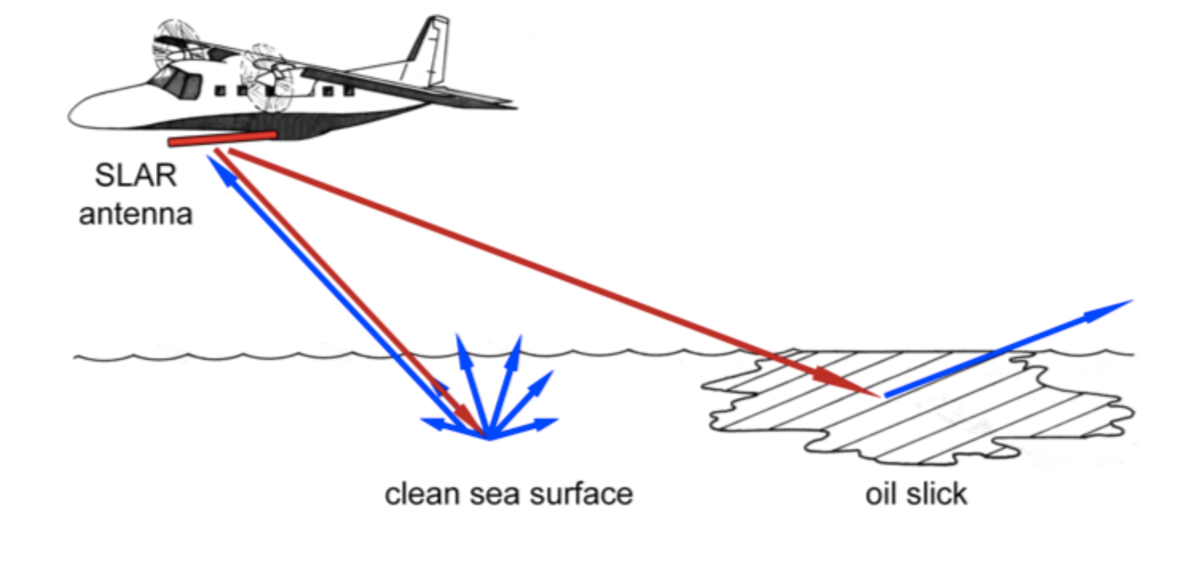
\includegraphics[scale=0.2]{img/section_03/sar-petroleo.png}
        \caption{Dinámica de la interacción entre el pulso del radar y la superficie del derrame de petróleo}
        \label{fig:section_03_dinamica_sar_petroleo}
    \end{figure}
\end{frame}


\section{Bases de Datos}
\begin{frame}{Problemáticas}
    \begin{itemize}
        \item No existe en la literatura un conjunto estandarizado.

        \item Los datasets generalmente no se encuentran disponibles.

        \item La segmentación no es muy precisa.        
    \end{itemize}
\end{frame}

\begin{frame}{Datasets (no todos son de derrames)}
    \footnotesize
    \begin{itemize}
        \item Oil Spill Dataset \href{https://m4d.iti.gr/oil-spill-detection-dataset/}{https://m4d.iti.gr/oil-spill-detection-dataset/}
        
        Contains jpg images extracted from satellite Synthetic Aperture Radar (SAR) data depicting oil spills and other relevant instances, as well as their corresponding ground truth masks. The developed dataset (~400MB) contains around 1000 images for training and 110 images for testing, depicting instances of 5 classes, namely oil spill, look-alike, land, ship and sea areas. \cite{rs11151762}
        
        \item SOS \href{http://cugurs5477.mikecrm.com/5tk5gyO}{http://cugurs5477.mikecrm.com/5tk5gyO}
    
        This data set has two study areas, the Gulf of Mexico oil spill area and the Persian Gulf oil spill area. 
        It is a pixel-level data set of oil spill and non-oil spill,and is made available for research purposes only. 
        PALSAR images were used in the Gulf of Mexico study area. Sentinel 1A images were used for the Persian Gulf study area. \cite{9568691}
        
        \item CHN6 CUG \href{http://cugurs5477.mikecrm.com/ZtMn5tR}{http://cugurs5477.mikecrm.com/ZtMn5tR}
        
        This dataset is a pixel level high-resolution satellite image with artificial label and 6 representative cities in China are selected. CHN6-CUG contains 4511 labeled images of 512×512 size, divided into 3608 for model training and 903 for testing and result evaluation, with a resolution of 50 cm/pixel. \cite{Zhu2021AGC}
    \end{itemize}
\end{frame}
%
%\begin{frame}
%\frametitle{Oil Spill Dataset}
%    Oil Spill Identification from Satellite Images Using Deep Neural Network
%    \cite{rs11151762}
%    \begin{figure}
%        \centering
%        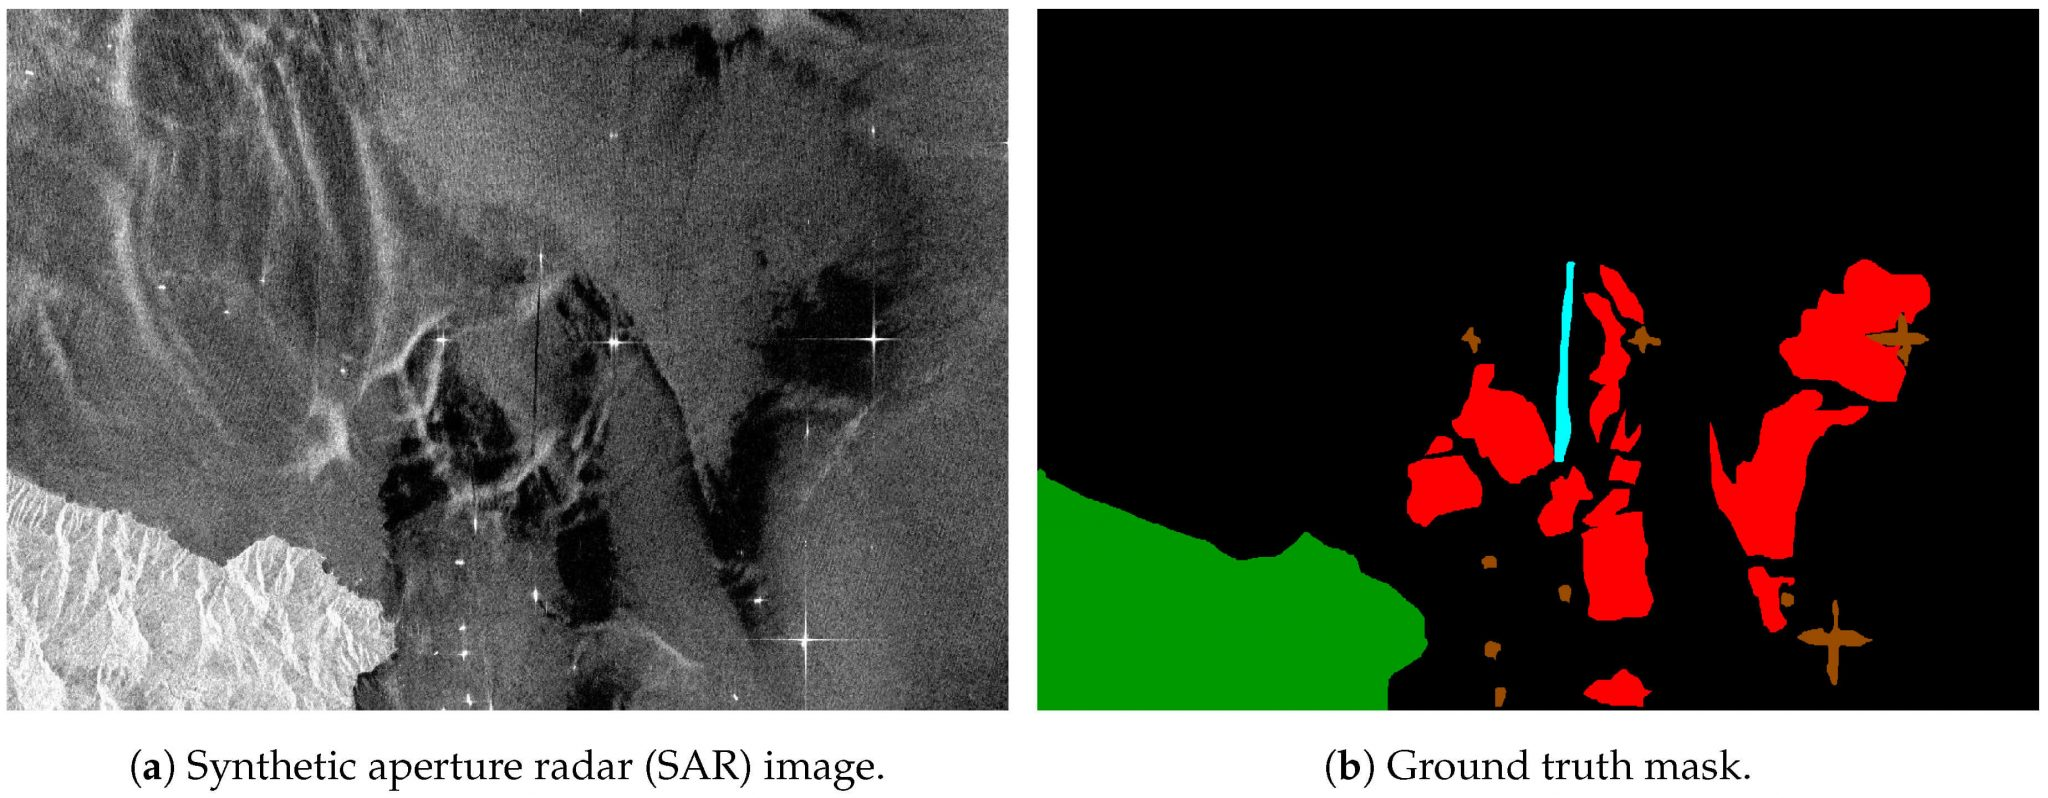
\includegraphics[scale=0.2]{img/section_04/oil_spill_dataset.jpg}
%        \caption{Oil Spill Dataset}
%        \label{fig:section2_oil_spill_dataset}
%    \end{figure}
%\end{frame}
%
%\begin{frame}
%\frametitle{Oil Spill Dataset}
%    Oil Spill Identification from Satellite Images Using Deep Neural Network
%    \cite{rs11151762}
%    \begin{figure}
%        \centering
%        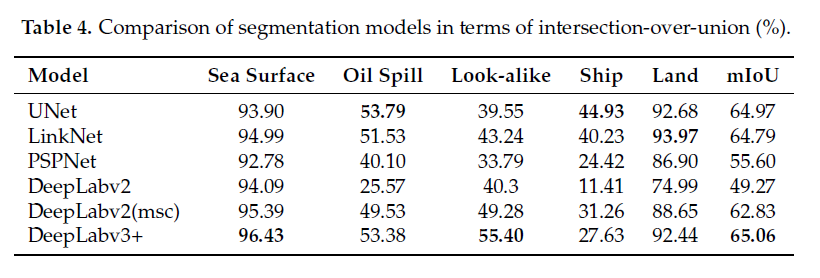
\includegraphics[scale=0.5]{img/section_04/krestenitis_results.png}
%        \caption{Resultados Oil Spill Dataset}
%        \label{fig:section2_oil_spill_dataset}
%    \end{figure}
%\end{frame}
%
%\begin{frame}
%\frametitle{CHN6-CUG}
%    A Global Context-aware and Batch-independent Network for road extraction from VHR satellite imagery
%    \cite{Zhu2021AGC}
%    \begin{figure}
%        \centering
%        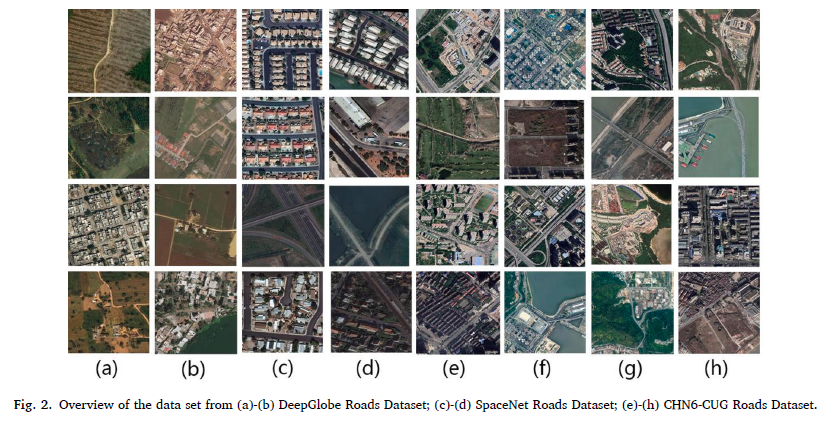
\includegraphics[scale=0.6]{img/section_04/chn6_01.png}
%        \caption{CHN6-CUG}
%        \label{fig:section2_chn6}
%    \end{figure}
%\end{frame}
%
%\begin{frame}
%\frametitle{SOS}
%    Oil Spill Contextual and Boundary-Supervised Detection Network Based on Marine SAR Images
%    \cite{9568691}
%    \begin{figure}
%        \centering
%        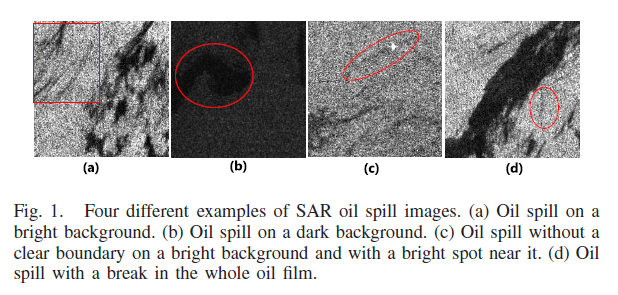
\includegraphics[scale=0.6]{img/section_04/sos_01.png}
%        \caption{SOS}
%        \label{fig:section2_sos}
%    \end{figure}
%\end{frame}
%
%\begin{frame}
%\frametitle{SOS}
%    Oil Spill Contextual and Boundary-Supervised Detection Network Based on Marine SAR Images
%    \cite{9568691}
%    \begin{figure}
%        \centering
%        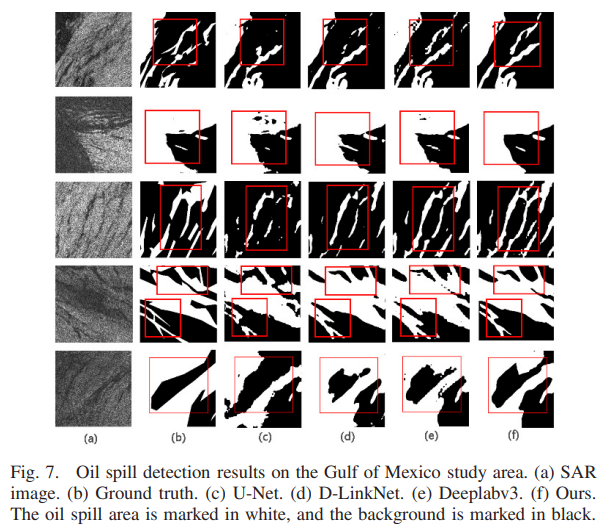
\includegraphics[scale=0.4]{img/section_04/sos_segmentation_01.png}
%        \caption{SOS}
%        \label{fig:section4_sos_segmentation_01}
%    \end{figure}
%\end{frame}
%
%\begin{frame}
%\frametitle{SOS}
%    Oil Spill Contextual and Boundary-Supervised Detection Network Based on Marine SAR Images
%    \cite{9568691}
%    \begin{figure}
%        \centering
%        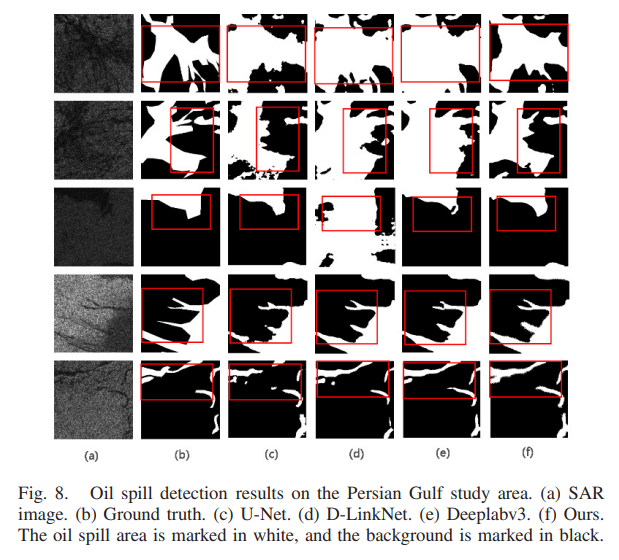
\includegraphics[scale=0.4]{img/section_04/sos_segmentation_02.png}
%        \caption{SOS}
%        \label{fig:section4_sos_segmentation_02}
%    \end{figure}
%\end{frame}
%
%\begin{frame}{Dataset CIMAT}
%    Preprocesamiento de canales de varianza y campo de viento para complementar la información de la imagen original (SAR) con los valores de la retrodispersión
%
%    \begin{figure}
%        \centering
%        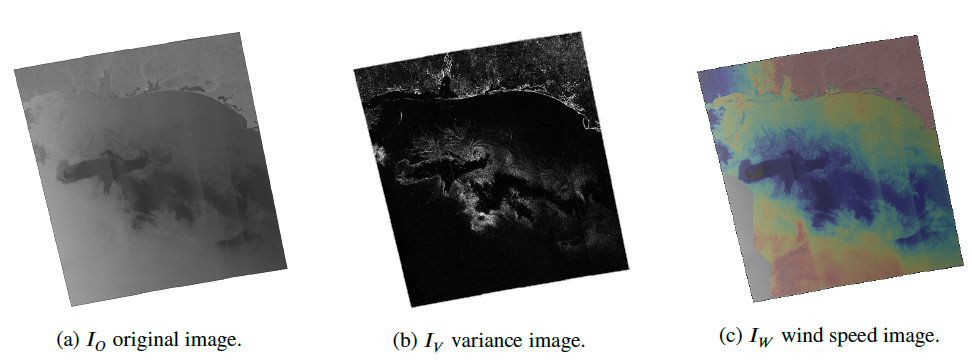
\includegraphics[scale=0.5]{img/section_04/canales.png}
%        \caption{Canales de entrada}
%        \label{fig:my_label}
%    \end{figure}
%\end{frame}
%
%\begin{frame}{Campo de viento}
%    \footnotesize
%    \begin{itemize}
%        \item El campo de viento proporciona información asociada a la rugosidad superficial del océano, ya que si existe poca intensidad de viento las manchas podrán ser visibles teniendo un fondo oscuro mas homogéneo.
%        \item Si la intensidad del viento es demasiado alta la mancha se dispersa y se degrada en el océano.
%    \end{itemize}
%
%    \begin{figure}
%        \centering
%        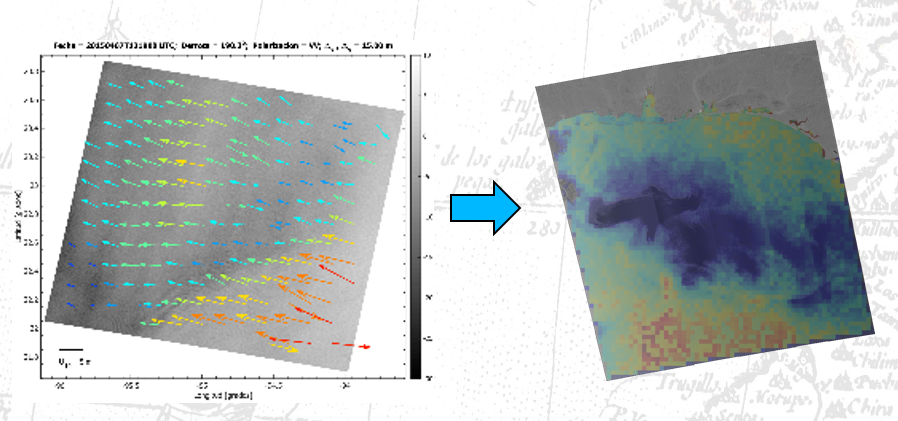
\includegraphics[scale=0.3]{img/section_04/campo_viento.png}
%        \caption{Campo de viento}
%        \label{fig:enter-label}
%    \end{figure}
%\end{frame}
%
%\begin{frame}{Subimágenes}
%    \begin{figure}
%        \centering
%        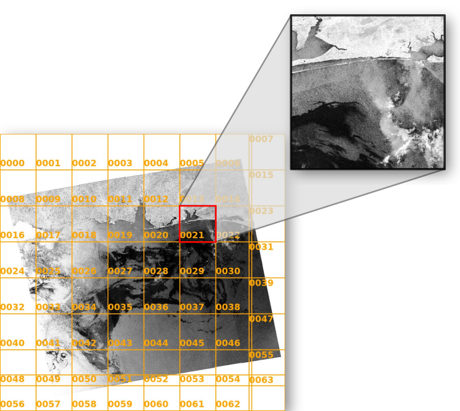
\includegraphics[scale=0.4]{img/section_04/subimagenes.png}
%        \caption{Generación de subimágenes}
%        \label{fig:enter-label}
%    \end{figure}
%\end{frame}
%
%\begin{frame}
%\frametitle{Segmentación Multicanal}
%    \begin{figure}
%        \centering
%        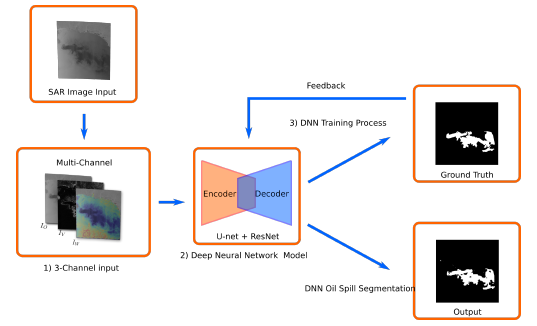
\includegraphics[scale=0.5]{img/section_04/pipeline.png}
%        \caption{Esquema general de la segmentación}
%        \label{fig:my_label}
%    \end{figure}
%\end{frame}
%


\section{Redes Profundas para Segmentación}
\begin{frame}[allowframebreaks]
\frametitle{Arquitecturas empleadas}

\begin{figure}[h!]
    \centering
    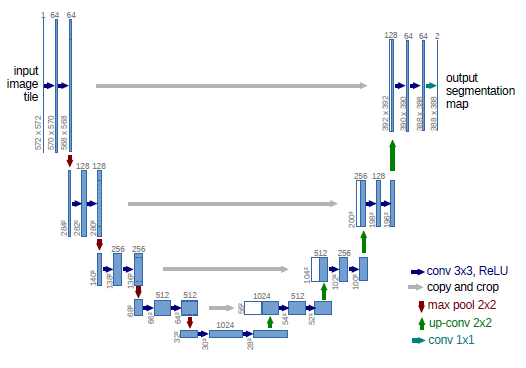
\includegraphics[scale=0.5]{img/section_05/unet-architecture.png}
    \caption{U-net \cite{DBLP:journals/corr/RonnebergerFB15}}
    \label{fig:unet-architecture}
\end{figure}

%\begin{figure}[h!]
%    \centering
%    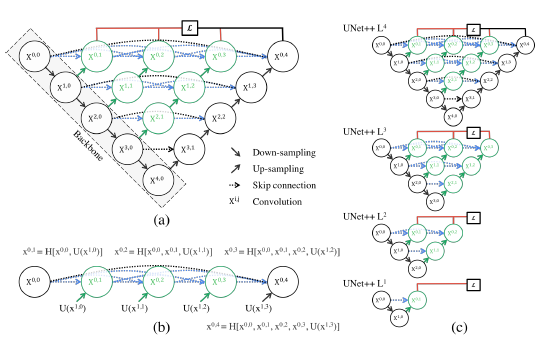
\includegraphics[scale=0.5]{img/section_05/unet-pp-architecture.png}
%    \caption{UNet++ \cite{DBLP:journals/corr/abs-1807-10165}}
%    \label{fig:unet-pp-architecture}
%\end{figure}

\begin{figure}[h!]
    \centering
    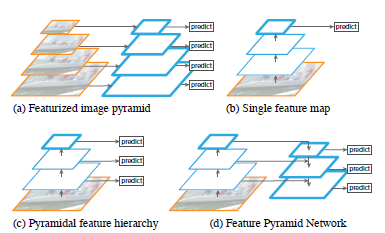
\includegraphics[scale=0.5]{img/section_05/fpn-architecture.png}
    \caption{Feature Pyramid Network (FPN) \cite{DBLP:journals/corr/LinDGHHB16}}
    \label{fig:fpn-architecture}
\end{figure}

\begin{figure}[h!]
    \centering
    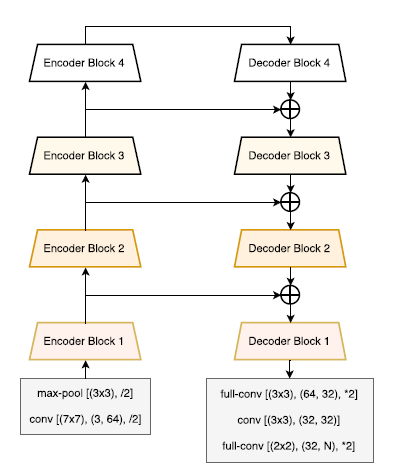
\includegraphics[scale=0.5]{img/section_05/linknet-architecture.png}
    \caption{LinkNet \cite{DBLP:journals/corr/ChaurasiaC17}}
    \label{fig:linknet-architecture}
\end{figure}

%\begin{figure}[h!]
%    \centering
%    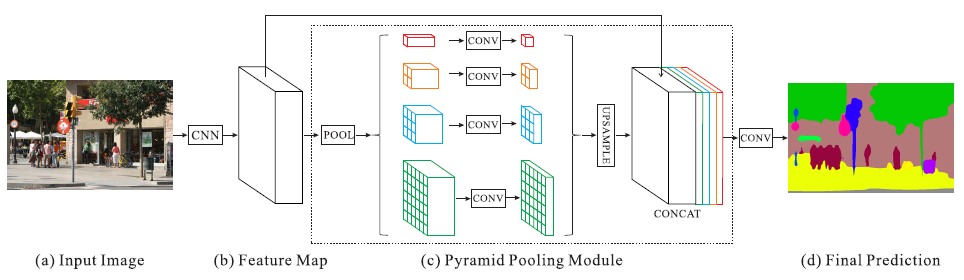
\includegraphics[scale=0.4]{img/section_05/PSPNet.png}
%    \caption{PSPNet \cite{DBLP:journals/corr/ZhaoSQWJ16}}
%    \label{fig:pspnet-architecture}
%\end{figure}

%\begin{figure}[h!]
%    \centering
%    \includegraphics[scale=0.6]{img/section_05/pan-architecture.png}
%    \caption{PAN \cite{DBLP:journals/corr/abs-1805-10180}}
%    \label{fig:pan-architecture}
%\end{figure}

%\begin{figure}
%    \centering
%    \includegraphics[scale=0.6]{img/section_05/pan-modules.png}
%    \caption{PAN \cite{DBLP:journals/corr/abs-1805-10180}}
%    \label{fig:pan-modules}
%\end{figure}

%\begin{figure}
%    \centering
%    \includegraphics{img/section_05/pan-global-attention-upsample.png}
%    \caption{Global Attention Upsample \cite{DBLP:journals/corr/abs-1805-%10180}}
%    \label{fig:pan-global-attention-upsample}
%\end{figure}

%\begin{figure}[h!]
%    \centering
%    \includegraphics[scale=0.6]{img/section_05/manet-architecture.png}
%    \caption{MANet \cite{9201310}}
%    \label{fig:manet-architecture}
%\end{figure}

\end{frame}


%\section{Resultados Comparativos}
%\begin{frame}
\frametitle{Resultados de la Segmentación en Oil Spill Dataset}

\begin{itemize}
    \item UNet (30 épocas)
\end{itemize}    
    \begin{table}[]
        \centering
        \small
        \begin{tabular}{l|c|c|c}
            \hline
            Backbone        & Loss    & IoU     & F1 \\
            \hline
            VGG16           & 0.45566 & 0.50114 & 0.40113 \\
            VGG19           & 0.44587 & 0.40173 & 0.50689 \\
            ResNet18        & 0.43212 & 0.41164 & 0.51881 \\
            ResNext50       & 0.40226 & 0.44552 & 0.54420 \\ 
            InceptionV3     & \textbf{0.37950} & \textbf{0.46721} & \textbf{0.56968} \\
            DenseNet121     & 0.38590 & 0.45168 & 0.55749 \\
            SEResNet18      & 0.43127 & 0.42239 & 0.52734 \\
            MobileNet       & 0.39336 & 0.44545 & 0.54890 \\ 
            MobileNet V2    & 0.51077 & 0.35173 & 0.46304 \\
            EfficientNetB0  & 0.38767 & 0.44784 & 0.55184 \\
            EfficientNetB1  & 0.38988 & 0.45152 & 0.55382 \\
            \hline
        \end{tabular}
        \caption{Resultados del entrenamiento con UNet}
        \label{tab:my_label}
    \end{table}
\end{frame}

\begin{frame}
\frametitle{Resultados de la segmentación - Oil Spill Dataset}
\begin{itemize}
    \item UNet (InceptionV3)
\end{itemize}    
\begin{figure}
    \centering
    \begin{tabular}{cc}
         \includegraphics[scale=0.15]{img/section_06/unet_inceptionv3_resultado_01.png}&&
         \includegraphics[scale=0.15]{img/section_06/unet_inceptionv3_resultado_02.png}\\
         \includegraphics[scale=0.12]{img/section_06/unet_inceptionv3_training_results.png}
    \end{tabular}
    \caption{Resultados de la segmentación UNet (30 épocas)}
    \label{fig:my_label}
\end{figure}
\end{frame}

\begin{frame}
\frametitle{Resultados de la Segmentación en Oil Spill Dataset}

\begin{itemize}
    \item UNet (50 épocas)
\end{itemize}    
    \begin{table}[]
        \centering
        \small
        \begin{tabular}{l|c|c|c}
            \hline
            Backbone        & Loss    & IoU     & F1 \\
            \hline
            VGG16           & 0.38731 & 0.44790 & 0.54889 \\
            VGG19           & 0.40118 & 0.43932 & 0.53753 \\
            ResNet18        & 0.36104 & 0.46592 & 0.56925 \\
            ResNext50       & \textbf{0.35660} & 0.47251 & \textbf{0.57368} \\ 
            InceptionV3     & 0.36673 & 0.46643 & 0.56779 \\
            DenseNet121     & 0.37890 & 0.45305 & 0.55465 \\
            SEResNet18      & 0.39182 & 0.44560 & 0.54850 \\
            MobileNet       & 0.37857 & 0.45648 & 0.55577 \\ 
            MobileNet V2    & 0.37603 & 0.45685 & 0.55593 \\
            EfficientNetB0  & 0.36888 & 0.45906 & 0.56276 \\
            EfficientNetB1  & 0.37087 & 0.45949 & 0.56217 \\
            EfficientNetB3  & 0.36485 & 0.46378 & 0.56617 \\
            EfficientNetB3  & 0.35709 & \textbf{0.47356} & 0.57298 \\
            \hline
        \end{tabular}
        \caption{Resultados del entrenamiento con UNet}
        \label{tab:my_label}
    \end{table}

\end{frame}

\begin{frame}
\frametitle{Resultados de la segmentación - Oil Spill Dataset}
\begin{itemize}
    \item UNet(EfficientNetB3)
\end{itemize}    

\begin{figure}
    \centering
    \begin{tabular}{cc}
         \includegraphics[scale=0.15]{img/section_06/unet50/efficientnetb3_resultado77.png}&&
         \includegraphics[scale=0.15]{img/section_06/unet50/efficientnetb3_resultado98.png}\\
         \includegraphics[scale=0.12]{img/section_06/unet50/efficientnetb3_training_results.png}
    \end{tabular}
    \caption{Resultados de la segmentación UNet (50 épocas)}
    \label{fig:my_label}
\end{figure}
\end{frame}

\begin{frame}
\frametitle{Resultados de la Segmentación en Oil Spill Dataset}

\begin{itemize}
    \item LinkNet (30 épocas)
\end{itemize}
    \begin{table}[]
        \centering
        \small
        \begin{tabular}{l|c|c|c}
            \hline
            Backbone        & Loss    & IoU     & F1 \\
            \hline
            VGG16           & 0.51160 & 0.35445 & 0.46811 \\
            VGG19           & 0.50209 & 0.35656 & 0.46109 \\
            ResNet18        & 0.42136 & 0.41926 & 0.52544 \\
            ResNext50       & 0.43413 & 0.41151 & 0.52428 \\ 
            InceptionV3     & 0.41608 & 0.42870 & 0.52965 \\
            DenseNet121     & 0.41567 & 0.43012 & 0.53101 \\
            SEResNet18      & 0.45467 & 0.39704 & 0.50374 \\
            MobileNet       & 0.42681 & 0.43919 & 0.54153 \\ 
            MobileNet V2    & 0.41577 & 0.43314 & 0.53733 \\
            EfficientNetB0  & 0.40657 & 0.43324 & 0.53863 \\
            EfficientNetB1  & \textbf{0.39538} & \textbf{0.44272} & \textbf{0.54845} \\
            \hline
        \end{tabular}
        \caption{Resultados del entrenamiento con LinkNet}
        \label{tab:my_label}
    \end{table}

\end{frame}

\begin{frame}
\frametitle{Resultados de la segmentación - Oil Spill Dataset}
\begin{itemize}
    \item LinkNet(EfficientNetB1)
\end{itemize}

\begin{figure}
    \centering
    \begin{tabular}{cc}
         \includegraphics[scale=0.15]{img/section_06/linknet_efficientnetb1_resultado_01.png}&&
         \includegraphics[scale=0.15]{img/section_06/linknet_efficientnetb1_resultado_02.png}\\
         \includegraphics[scale=0.12]{img/section_06/linknet_efficientnetb1_training_results.png}
    \end{tabular}
    \caption{Resultados de la segmentación LinkNet (30 épocas)}
    \label{fig:my_label}
\end{figure}
\end{frame}

\begin{frame}
\frametitle{Resultados de la Segmentación en Oil Spill Dataset}

\begin{itemize}
    \item LinkNet (50 épocas)
\end{itemize}
    \begin{table}[]
        \centering
        \small
        \begin{tabular}{l|c|c|c}
            \hline
            Backbone        & Loss    & IoU     & F1 \\
            \hline
            VGG16           & 0.40791 & 0.43255 & 0.53222 \\
            VGG19           & 0.39859 & 0.43914 & 0.54251 \\
            ResNet18        & 0.38332 & 0.44659 & 0.55128 \\
            ResNext50       & 0.36718 & 0.46303 & 0.56414 \\ 
            InceptionV3     & 0.36917 & 0.46123 & 0.56375 \\
            DenseNet121     & 0.39278 & 0.44348 & 0.54520 \\
            SEResNet18      & 0.40440 & 0.42711 & 0.53362 \\
            MobileNet       & 0.37634 & 0.45620 & 0.55743 \\ 
            MobileNet V2    & 0.38189 & 0.44708 & 0.55195 \\
            EfficientNetB0  & 0.37580 & 0.45786 & 0.56070 \\
            EfficientNetB1  & 0.36264 & \textbf{0.46611} & 0.56750 \\
            EfficientNetB2  & \textbf{0.35914} & 0.46599 & \textbf{0.56928} \\
            EfficientNetB1  & 0.37813 & 0.45397 & 0.55441 \\
            \hline
        \end{tabular}
        \caption{Resultados del entrenamiento con LinkNet}
        \label{tab:my_label}
    \end{table}
\end{frame}

\begin{frame}
\frametitle{Resultados de la segmentación - Oil Spill Dataset}
\begin{itemize}
    \item LinkNet(EfficientNetB1)
\end{itemize}
\begin{figure}
    \centering
    \begin{tabular}{cc}
         \includegraphics[scale=0.15]{img/section_06/linknet50/efficientnetb3_resultado103.png}&&
         \includegraphics[scale=0.15]{img/section_06/linknet50/efficientnetb3_resultado37.png}\\
         \includegraphics[scale=0.12]{img/section_06/linknet50/efficientnetb3_training_results.png}
    \end{tabular}
    \caption{Resultados de la segmentación LinkNet (50 épocas)}
    \label{fig:my_label}
\end{figure}
\end{frame}

\begin{frame}
\frametitle{Resultados de la Segmentación en Oil Spill Dataset}

\begin{itemize}
    \item FPN (30 épocas)
\end{itemize}
    
    \begin{table}[]
        \centering
        \small
        \begin{tabular}{l|c|c|c}
            \hline
            Backbone        & Loss    & IoU     & F1 \\
            \hline
            VGG16           & 0.38663 & 0.44950 & 0.55168 \\
            VGG19           & 0.39642 & 0.43647 & 0.54282 \\
            ResNet18        & 0.39412 & 0.43772 & 0.54311 \\
            ResNext50       & 0.39544 & 0.43457 & 0.54063 \\ 
            InceptionV3     & 0.38186 & 0.45064 & 0.55056 \\
            DenseNet121     & 0.40649 & 0.43112 & 0.53142 \\
            SEResNet18      & 0.39456 & 0.43615 & 0.54126 \\
            MobileNet       & 0.37814 & 0.45306 & 0.55631 \\ 
            MobileNet V2    & 0.39249 & 0.44255 & 0.54807 \\
            EfficientNetB0  & \textbf{0.37707} & \textbf{0.45358} & 0.55442 \\
            EfficientNetB1  & 0.38023 & 0.45093 & \textbf{0.55456} \\
            \hline
        \end{tabular}
        \caption{Resultados del entrenamiento con FPN}
        \label{tab:my_label}
    \end{table}
\end{frame}

\begin{frame}
\frametitle{Resultados de la segmentación - Oil Spill Dataset}
\begin{itemize}
    \item FPN(EfficientNetB0,B1)
\end{itemize}

\begin{figure}
    \centering
    \begin{tabular}{cc}
         \includegraphics[scale=0.15]{img/section_06/fpn_efficientnetb0_resultado_01.png}&&
         \includegraphics[scale=0.15]{img/section_06/fpn_efficientnetb1_resultado_02.png}\\
         \includegraphics[scale=0.12]{img/section_06/fpn_efficientnetb1_training_results.png}
    \end{tabular}
    \caption{Resultados de la segmentación FPN (30 épocas)}
    \label{fig:my_label}
\end{figure}
\end{frame}

\begin{frame}
\frametitle{Resultados de la Segmentación en Oil Spill Dataset}
\begin{itemize}
    \item FPN (50 épocas)
\end{itemize}
    \begin{table}[]
        \centering
        \small
        \begin{tabular}{l|c|c|c}
            \hline
            Backbone        & Loss    & IoU     & F1 \\
            \hline
            VGG16           & 0.38189 & 0.44954 & 0.55027 \\
            VGG19           & 0.37653 & 0.45591 & 0.55571 \\
            ResNet18        & 0.39561 & 0.44309 & 0.54304 \\
            ResNext50       & 0.36392 & 0.46511 & 0.56499 \\ 
            InceptionV3     & 0.39995 & 0.43918 & 0.53494 \\
            DenseNet121     & 0.37311 & 0.45484 & 0.55666 \\
            SEResNet18      & 0.38922 & 0.44315 & 0.54345 \\
            MobileNet       & 0.37649 & 0.45590 & 0.55584 \\ 
            MobileNet V2    & 0.37500 & 0.45930 & 0.56106 \\
            EfficientNetB0  & 0.36161 & 0.46685 & 0.56791 \\
            EfficientNetB1  & \textbf{0.34946} & \textbf{0.47850} & \textbf{0.57835} \\
            EfficientNetB2  & 0.35209 & 0.47497 & 0.57533 \\
            EfficientNetB3  & 0.37618 & 0.45351 & 0.55577 \\
            \hline
        \end{tabular}
        \caption{Resultados del entrenamiento con FPN}
        \label{tab:my_label}
    \end{table}
\end{frame}

\begin{frame}
\frametitle{Resultados de la segmentación - Oil Spill Dataset}
\begin{itemize}
    \item FPN(EfficientNetB1)
\end{itemize}
\begin{figure}
    \centering
    \begin{tabular}{cc}
         \includegraphics[scale=0.15]{img/section_06/fpn50/efficientnetb1_resultado73.png}&&
         \includegraphics[scale=0.15]{img/section_06/fpn50/efficientnetb1_resultado79.png}\\
         \includegraphics[scale=0.12]{img/section_06/fpn50/efficientnetb1_training_results.png}
    \end{tabular}
    \caption{Resultados de la segmentación FPN (50 épocas)}
    \label{fig:my_label}
\end{figure}
\end{frame}

\begin{frame}[allowframebreaks]
\frametitle{Resultados obtenidos (v2.0)}
\begin{table}[h!]
    \centering
    \begin{tabular}{|l|c|c|c|}
        \hline
        Arquitectura & Train IoU & Valid IoU & Test IoU \\
         \hline
        U-net & 0.953881502 & 0.829308152 & 0.810642958 \\
        UNet++ & 0.957234263 & 0.827012777 & 0.81362468 \\
        FPN & 0.958307505 & 0.825693786 & 0.81834054 \\
        LinkNet & 0.910990953 & 0.809995234 & 0.817955494 \\
        PSP & 0.952400804 & 0.784086466 & 0.784680903 \\
        PAN & 0.95680362 & 0.833234131 & 0.822393894 \\
        MANet & 0.954820871 & 0.820060194 & 0.814887702 \\
        \hline
    \end{tabular}
    \caption{Resultados Per Image}
    \label{tab:resultados_per_image}
\end{table}

\begin{table}[h!]
    \centering
    \begin{tabular}{|l|c|c|c|}
        \hline
        Arquitectura & Train IoU & Valid IoU & Test IoU \\
         \hline
        U-net & 0.925344884 & 0.425292462 & 0.362593859 \\
        UNet++ & 0.924023926 & 0.434665382 & 0.375736356 \\
        FPN & 0.919602633 & 0.421498924 & 0.394982636 \\
        LinkNet & 0.799012482 & 0.392058462 & 0.379849225 \\
        PSP & 0.908014834 & 0.394087285 & 0.33700341 \\
        PAN & 0.913587391 & 0.438524336 & 0.392617226 \\
        MANet & 0.911941469 & 0.430485725 & 0.406906128 \\
        \hline
    \end{tabular}
    \caption{Resultados Dataset}
    \label{tab:resultados_dataset}
\end{table}
\end{frame}

\begin{frame}{Dataset CIMAT}
    \tiny
    Linknet
    \centering
    \begin{tabular}{c|c|c|c|c}
         \hline        train accuracy&cross val accuracy&train loss&cross val loss&time\\
         \hline
0.9135&0.2292&0.2084&20.5706&0:15:25.9513  \\
0.9321&0.7309&0.1613&4.5319&0:08:14.0341  \\
0.9413&0.8682&0.1408&0.2849&0:07:53.0278  \\
0.9447&0.7840&0.1334&0.4378&0:07:34.2589  \\
0.9498&0.7721&0.1211&0.5060&0:07:41.0982  \\
0.9522&0.8335&0.1163&0.4812&0:07:54.5108  \\
0.9529&0.7936&0.1127&0.6172&0:07:37.0849  \\
0.9550&0.9173&0.1081&0.2430&0:07:41.8006  \\
0.9559&0.8718&0.1057&0.4472&0:07:38.0394  \\
0.9582&0.8431&0.1014&0.3682&0:07:37.8231  \\
0.9641&0.9478&0.0862&0.1308&0:07:39.1014  \\
0.9659&0.8145&0.0824&0.9081&0:07:40.1780  \\
0.9672&0.9262&0.0783&0.2671&0:07:59.4524  \\
0.9692&0.8943&0.0745&0.2832&0:08:12.5293  \\
0.9703&0.9489&0.0722&0.1341&0:08:00.8487  \\
0.9717&0.9359&0.0683&0.1597&0:07:56.9729  \\
0.9718&0.9362&0.0679&0.1630&0:07:55.0680  \\
0.9731&0.9241&0.0652&0.2339&0:08:09.4719  \\
0.9749&0.9226&0.0609&0.2082&0:07:51.4603  \\
0.9753&0.9173&0.0601&0.2194&0:07:51.9716  \\
    \hline
    \end{tabular}
\end{frame}

\begin{frame}{Dataset CIMAT}
    \tiny
    FPN
    \centering
    \begin{tabular}{c|c|c|c|c}
         \hline        train accuracy&cross val accuracy&train loss&cross val loss&time\\
         \hline
0.9165&0.3551&0.1959&1.3169&0:25:44.8352\\
0.9366&0.9120&0.1484&1.0141&0:25:21.0023\\
0.9443&0.7229&0.1331&0.7193&0:26:21.7031\\
0.9475&0.8190&0.1252&0.3640&0:25:38.0897\\
0.9503&0.7986&0.1196&0.8158&0:22:57.3958\\
0.9536&0.8073&0.1095&0.3852&0:22:17.9054\\
0.9557&0.9390&0.1061&0.1657&0:22:17.2939\\
0.9578&0.8955&0.1007&0.3413&0:23:30.5936\\
0.9598&0.9196&0.0968&0.1922&0:23:10.0042\\
0.9617&0.7772&0.0919&0.5507&0:22:56.4491\\
0.9686&0.9262&0.0752&0.1777&0:22:02.3274\\
0.9702&0.8144&0.0716&0.4685&0:22:35.3553\\
0.9710&0.9467&0.0702&0.1392&0:22:01.0859\\
0.9730&0.9246&0.0654&0.1819&0:22:46.4153\\
0.9743&0.9525&0.0622&0.1149&0:22:38.2599\\
0.9745&0.9491&0.0622&0.1321&0:22:08.8205\\
0.9765&0.8694&0.0575&0.4003&0:22:13.8110\\
0.9765&0.9356&0.0574&0.1699&0:22:26.7005\\
0.9787&0.9536&0.0518&0.1204&0:22:51.8932\\
0.9788&0.9442&0.0514&0.1805&0:22:26.3315\\
    \hline
    \end{tabular}
\end{frame}

\begin{frame}{Dataset CIMAT}
    \tiny
    Unet
    \centering
    \begin{tabular}{c|c|c|c|c}
         \hline        train accuracy&cross val accuracy&train loss&cross val loss&time\\
         \hline
0.9101&0.4451&0.2129&0.9967&0:12:56.3800\\
0.9325&0.8417&0.1623&0.3851&0:07:40.2358\\
0.9406&0.9341&0.1430&0.1676&0:08:16.7219\\
0.9444&0.8946&0.1328&0.2260&0:08:17.0713\\
0.9482&0.8929&0.1242&0.2676&0:08:38.0430\\
0.9485&0.8501&0.1232&0.4255&0:08:24.9761\\
0.9520&0.9087&0.1161&0.2259&0:08:39.0020\\
0.9553&0.8190&0.1076&0.5862&0:08:30.0524\\
0.9563&0.6377&0.1042&11.2629&0:08:45.2755\\
0.9568&0.9530&0.1035&0.1101&0:08:37.9279\\
0.9642&0.9583&0.0861&0.1000&0:09:02.1637\\
0.9665&0.9015&0.0813&0.2152&0:08:46.9740\\
0.9673&0.9459&0.0790&0.1331&0:08:40.7595\\
0.9690&0.8902&0.0743&0.3482&0:08:52.2270\\
0.9700&0.8937&0.0722&0.2625&0:08:38.5683\\
0.9713&0.9369&0.0696&0.1645&0:08:41.7734\\
0.9720&0.9055&0.0679&0.2149&0:08:51.5161\\
0.9733&0.9131&0.0649&0.2414&0:08:47.8855\\
0.9739&0.9447&0.0637&0.1410&0:08:42.8911\\
0.9753&0.8692&0.0603&0.3389&0:08:53.1651\\
\hline
    \end{tabular}
\end{frame}


\section{Trabajo actual}
\begin{frame}[allowframebreaks]
\frametitle{Arquitectura UNet}
    \begin{figure}
        \centering
        \includegraphics[scale=0.3]{img/section_07/UNet.png}
        \caption{Esquema base}
        \label{fig:unet-base}
    \end{figure}

    \begin{figure}
        \centering
        \includegraphics[scale=0.3]{img/section_07/ResUNet.png}
        \caption{Conexiones residuales}
        \label{fig:res-unet}
    \end{figure}

    \begin{figure}
        \centering
        \includegraphics[scale=0.3]{img/section_07/Attention_UNet.png}
        \caption{Atención}
        \label{fig:attn-unet}
    \end{figure}

    \begin{figure}
        \centering
        \includegraphics[scale=0.3]{img/section_07/Attention_ResUNet.png}
        \caption{Atención + Conexiones residuales}
        \label{fig:att-res-unet}
    \end{figure}
\end{frame}

\begin{frame}{Transformada Wavelet}
    Las wavelets son señales, o formas de onda, las cuales tienen una duración limitada y un valor promedio de cero. Las wavelets pueden ser irregulares y asimétricas, características que les otorgan una mejor adaptación en el análisis de señales en comparación con la transformada de Fourier.

    \begin{figure}
        \centering
        \includegraphics[scale=0.3]{img/section_07/Symlet-4.jpg}
        \caption{Symlet 4}
        \label{fig:symlet4}
    \end{figure}
\end{frame}

\begin{frame}
    De forma general la transformada wavelet descompone una señal mediante el uso de las versiones escaladas y desplazadas de la wavelet madre.

    \begin{figure}
        \centering
        \includegraphics[scale=0.3]{img/section_07/Filtros.jpg}
        \caption{Filtros}
        \label{fig:filtros}
    \end{figure}
\end{frame}

\begin{frame}{Descomposición por Wavelets}
    \begin{figure}
        \centering
        \includegraphics[scale=0.4]{img/section_07/Wavelets_decomposition.png}
        \caption{Descomposición por Wavelets}
        \label{fig:descomposicion}
    \end{figure}
\end{frame}

\begin{frame}{Retos}
    \begin{figure}
    \centering
    \begin{tabular}{cc}
         \includegraphics[scale=0.45]{img/section_07/derrame.jpg} &
         \includegraphics[scale=0.15]{img/section_07/campo_viento.jpg}\\
         \includegraphics[scale=0.15]{img/section_07/segmentacion_01.jpg}& 
         \includegraphics[scale=0.15]{img/section_07/segmentacion_02.jpg}
    \end{tabular}
    \caption{Resultado de la segmentación en Sentinel 1}
    \label{fig:my_label}
\end{figure}
\end{frame}

\begin{frame}{Retos}
    \begin{figure}
        \centering
        \includegraphics[scale=0.3]{img/section_07/segmentacion_03.jpg}
        \caption{Falsos positivos}
        \label{fig:enter-label}
    \end{figure}
\end{frame}

\begin{frame}{Retos}
    \begin{itemize}
        \item Ampliación del dataset.- el entrenamiento se ha realizado con un conjunto de imágenes Envisat.
        
        \item Entrenamiento distribuido.- cada iteración con el dataset (~80,000 imágenes) tarda aproximadamente entre 30 y 40 minutos.
        
        \item Integración de canales adicionales.- bandas multiespectrales e hiperespectrales.        
        \item Integración de otros marcos de descomposición (ridgelets, curvlets, shearlets)
    \end{itemize}
\end{frame}


%%%%%%%% referencias %%%%%%%%
\nocite{*}
\begin{frame}[allowframebreaks]{Referencias}
\bibliographystyle{unsrt}
\bibliography{ref.bib}
\end{frame}

\end{document}
